%Document-Author: Nicoletti Luca + Padovan Tommaso
%Document-Date: 2016/01/13
%Document-Description: Documento di Piano di Progetto del gruppo SWEeneyThreads 

\documentclass[a4paper]{report}
\usepackage[english, italian]{babel}
\usepackage[T1]{fontenc}
\usepackage[utf8]{inputenc}
\usepackage{url}
\usepackage{graphicx}
\usepackage[hidelinks]{hyperref}
\usepackage{booktabs}
\usepackage{eurosym}
\usepackage{tabularx}
\usepackage{pifont}
\usepackage[table]{xcolor}
\usepackage{float}
\usepackage[]{appendix}
\usepackage{ltxtable} 
\usepackage{geometry}
\geometry{margin=1in}
\usepackage{longtable}
\usepackage{multirow}

\graphicspath{{Immagini/}}

\newcolumntype{Y}{>{\centering\arraybackslash}X}
\newcolumntype{s}{>{\hsize=.21\hsize}X}
\newcolumntype{f}{>{\hsize=.37\hsize}X}
\newcolumntype{m}{>{\hsize=.42\hsize}X}
\newcolumntype{t}{>{\hsize=.1\hsize}X}
\newcolumntype{r}{>{\hsize=.3\hsize}X}
\newcolumntype{k}{>{\hsize=.4\hsize}X}

\newcommand{\mychapter}[2]{
	\setcounter{chapter}{#1}
	\setcounter{section}{0}
	\setcounter{subsection}{1}
	\chapter*{#2}
	\addcontentsline{toc}{chapter}{#2}
}

\renewcommand{\abstractname}{Tabella contenuti}

\begin{document}

	\begin{titlepage}
		% Defines a new command for the horizontal lines, change thickness here
		\newcommand{\HRule}{\rule{\linewidth}{0.5mm}} 
		\center  
		
		% HEADING SECTION
		\textsc{\LARGE SweeneyThreads}\\[1.5cm] 
		\textsc{\Large Actorbase}\\[0.5cm] 
		\textsc{\large a NoSQL DB based on the Actor model}\\[0.5cm]
		
		
		% TITLE SECTION
		\HRule \\[0.4cm]
		{ \huge \bfseries Piano di progetto}\\[0.4cm] 
		\HRule \\[1.5cm]
		
		% AUTHOR SECTION
		\begin{minipage}{0.4\textwidth}
			\begin{flushleft} \large
				\emph{Redattori:}\\
				Nicoletti \textsc{Luca} \\
				Padovan \textsc{Tommaso} \\
			\end{flushleft}
		\end{minipage}
		~
		\begin{minipage}{0.4\textwidth}
			\begin{flushright} \large
				\emph{Approvazione:} \\
				\dots \\
				\emph{Verifica:} \\
				Biggeri \textsc{Mattia} \\
				Tommasin \textsc{Davide} \\
			\end{flushright}
		\end{minipage}
		
		%immagine
		\begin{figure}[H]
			\centering
			
\includegraphics[scale=0.8]{sweeney.png}
		\end{figure}
		\begin{center}
			Versione 1.2.0
		\end{center}
		% Date, change the \today to a set date if you want to be precise
		{\large \today}\\[3cm] 
		% Fill the rest of the page with whitespace
		\vfill  
	\end{titlepage}
	
	\tableofcontents
	
	\mychapter{0}{Diario delle modifiche}
		\begin{table}[H]
			\begin{tabularx}{\textwidth}{sfmX}
				\noalign{\hrule height 1.5pt}
				\rowcolor{orange!85} Versione & Data & Autore & Descrizione \\
				\noalign{\hrule height 1.5pt}
				1.2.0 & 2016-01-20 & \emph{Responsabile} \newline Padovan Tommaso &  Approvazione documento \\
				\noalign{\hrule height 0.5pt}
				1.1.2 & 2016-01-19 & \emph{Amministratore} \newline Nicoletti Luca &  Inseriti i riferimenti \\
				\noalign{\hrule height 0.5pt}
				1.1.1 & 2016-01-18 & \emph{Amministratori} \newline Nicoletti Luca , \newline Padovan Tommaso &  Apportate le 
				modifiche rilevate necessarie dai Verificatori \\
				\noalign{\hrule height 0.5pt}
				1.1.0 & 2016-01-18 & \emph{Verificatori} \newline Biggeri Mattia , \newline Tommasin Davide &  Verificato il 
				documento, assegnato ai responsabili una lista di sistemazioni da apportare\\
				\noalign{\hrule height 0.5pt}
				1.0.6 & 2016-01-18 & \emph{Amministratore} \newline Nicoletti Luca , \newline Padovan Tommaso &  Inserite 
				le caption ad ogni tabella, inseriti i Gantt per ogni fase, \\
				\noalign{\hrule height 0.5pt}
				1.0.5 & 2016-01-17 & \emph{Amministratore} \newline Nicoletti Luca &  Inseriti tabelle costi 
				e riviste suddivisioni. Inseriti grafici dei costi\\
				\noalign{\hrule height 0.5pt}
				1.0.4 & 2016-01-17 & \emph{Amministratore} \newline Nicoletti Luca &  Inserite tabelle e programmata 
				l'intera durata del progetto\\
				\noalign{\hrule height 0.5pt}
				1.0.3 & 2016-01-16 & \emph{Amministratori} \newline Nicoletti Luca, \newline Padovan Tommaso & Inserita 
				introduzione alla Rendicontazione e inserita la descrizione di tutta la macro-fase di Analisi \\
				\noalign{\hrule height 0.5pt}
				1.0.2 & 2016-01-15 & \emph{Amministratore} \newline Nicoletti Luca & Inserita introduzione alla 
				Pianificazione e correzioni da verifica \\
				\noalign{\hrule height 0.5pt}
				1.0.1 & 2016-01-14 & \emph{Amministratore} \newline Nicoletti Luca & Stesura analisi dei rischi e 
				introduzione del documento \\
				\noalign{\hrule height 0.5pt}
				1.0.0 & 2016-01-13 & \emph{Amministratore} \newline Nicoletti Luca & Scrittura scheletro logico del documento \\
				\noalign{\hrule height 1.5pt}
			\end{tabularx}
			\caption{Diario delle modifiche } 
			\label{DModifiche}
		\end{table}
	
	\begin{appendices}
	\mychapter{1}{Organigramma}
		\section{Redazione}
		\begin{table}[H]
			\begin{tabularx}{\textwidth}{Y Y Y}
				\noalign{\hrule height 1.5pt}
				\rowcolor{orange!85}Nominativo & Data di redazione & Firma\\
				\noalign{\hrule height 1.5pt}
				Nicoletti Luca & 2016-01-13 & \\
				\noalign{\hrule height 0.5pt}
				Padovan Tommaso & 2016-01-13 &\\
				\noalign{\hrule height 1.5pt}
			\end{tabularx}
			\caption{Redazione documento } 
			\label{RedDocumento}
		\end{table}
		\section{Approvazione}
		\begin{table}[H]
			\begin{tabularx}{\textwidth}{Y Y Y}
				\noalign{\hrule height 1.5pt}
				\rowcolor{orange!85}Nominativo & Data di redazione & Firma\\
				\noalign{\hrule height 1.5pt}
				Nicoletti Luca & 2016-01-13 & \\
				\noalign{\hrule height 0.5pt}
				Padovan Tommaso & 2016-01-13 & \\
				\noalign{\hrule height 0.5pt}
				Prof. Vardanega Tullio & & \\
				\noalign{\hrule height 1.5pt}
			\end{tabularx}
			\caption{Approvazione documento } 
			\label{AppDocumento}
		\end{table}
		\section{Componenti}
		\begin{table}[H]
			\begin{tabularx}{\textwidth}{r r k}
				\noalign{\hrule height 1.5pt}
				\rowcolor{orange!85}Nominativo & Matricola & E-mail \\
				\noalign{\hrule height 1.5pt}
				Paolo Bonato & 1023655 & paolo.bonato.3@studenti.unipd.it\\
				\noalign{\hrule height 0.5pt}
				Matteo Bortolazzo & 1073194 & matteo.bortolazzo.1@studenti.unipd.it \\
				\noalign{\hrule height 0.5pt}
				Mattia Biggeri & 1074269 & mattia.biggeri@studenti.unipd.it \\
				\noalign{\hrule height 0.5pt}
				Elia Maino & 1069880 & elia.maino@studenti.unipd.it \\
				\noalign{\hrule height 0.5pt}
				Luca Nicoletti & 1070634 & luca.nicoletti.2@studenti.unipd.it \\
				\noalign{\hrule height 0.5pt}
				Tommaso Padovan & 1054128 & tommaso.padovan@studenti.unipd.it \\
				\noalign{\hrule height 0.5pt}
				Davide Tommasin & 1073541 & davide.tommasin.1@studenti.unipd.it \\
				\noalign{\hrule height 1.5pt}
			\end{tabularx}
			\caption{Componenti SWEeneyThreads } 
			\label{ComponentiGruppo}
		\end{table}
		\section{Accetazione componenti}
		\begin{table}[H]
			\begin{tabularx}{\textwidth}{Y Y Y}
				\noalign{\hrule height 1.5pt}
				\rowcolor{orange!85}Nominativo & Data di accettazione & Firma\\
				\noalign{\hrule height 1.5pt}
				Paolo Bonato & 2015-18-12 & \\
				\noalign{\hrule height 0.5pt}
				Matteo Bortolazzo & 2015-18-12 & \\
				\noalign{\hrule height 0.5pt}
				Mattia Biggeri & 2015-18-12 & \\
				\noalign{\hrule height 0.5pt}
				Elia Maino & 2015-18-12 & \\
				\noalign{\hrule height 0.5pt}
				Luca Nicoletti & 2015-18-12 & \\
				\noalign{\hrule height 0.5pt}
				Tommaso Padovan & 2015-18-12 & \\
				\noalign{\hrule height 0.5pt}
				Davide Tommasin & 2015-18-12 & \\
				\noalign{\hrule height 1.5pt}
			\end{tabularx}
			\caption{Accettazione componenti } 
			\label{AccComponenti}
		\end{table}
		\section{Definizione dei ruoli}
			Nel corso dello sviluppo del progetto i membri del gruppo dovranno ricoprire diversi ruoli, rappresentanti 
			figure aziendali specializzate, indispensabili per il buon esito del progetto. Ogni singolo componente del 
			gruppo può ricoprire più ruoli, sia contemporaneamente che in distinte fasi del progetto in ogni caso 
			sempre garantendo assenza di conflitto di interesse tra i ruoli assunti.
			Tali ruoli sono:
			\begin{itemize}
				\item \textbf{Responsabile:} Il \emph{Responsabile} rappresenta il progetto presso il fornitore e presso 
				il committente, accentrando le responsabilità di scelta e approvazione e partecipando al progetto per tutta 
				la sua durata. Ha responsabilità di pianificazione (elabora ed emana piani e scadenze), di gestione delle 
				risorse umane e di controllo, coordinamento e gestione delle relazioni esterne. Inoltre approva l'emissione 
				dei documenti, coordina le attività del gruppo e si relaziona con il controllo di qualità all'interno del 
				progetto. Per quanto riguarda la documentazione il responsabile redige l'\emph{organigramma} e il 
				\emph{Piano di progetto} oltre ad approvare l'offerta e i relativi allegati.
				\item \textbf{Amministratore:} L'\emph{Amministratore} si occupa dell'efficienza e dell'operatività dell'ambiente 
				di lavoro gestendo risorse, processi e infrastrutture.È inoltre responsabile della redazione e attuazione di piani 
				e procedure di Gestione per la Qualità, controlla versioni e configurazioni del prodotto e gestisce l'archivio 
				della documentazione di progetto (librarian). Per quanto riguarda la documentazione l'\emph{Amministratore} 
				collabora alla redazione del \emph{Piano di progetto} e redige le \emph{Norme di progetto} per conto del responsabile.
				\item \textbf{Analista:} Il compito principale dell'analista è capire il problema (non fornire una soluzione),
				tale compito è di importanza fondamentale poichè se il problema viene compreso in modo errato tutto il progetto 
				è destinato a fallire. L'\emph{Analista} deve conoscere il dominio del problema e avere una vasta esperienza professionale, 
				in genere un progetto prevede pochi analisti ed essi raramente seguono il progetto fino alla conclusione. Per 
				quanto riguarda la documentazione l'\emph{Analista} redige lo studio di fattibilità (un documento interno al gruppo) 
				e l'\emph{Analisi dei requisiti}.
				\item \textbf{Progettista:} Il compito del \emph{Progettista} è trovare una soluzione (eventualmente tra le tante disponibili) 
				ed assumersi la responsabilità della decisione presa. I progettisti hanno competenze tecniche e tecnologiche aggiornate 
				ed ampia esperienza professionale, influiscono fortemente sugli aspetti tecnici e tecnologici del progetto e spesso 
				ne assumono responsabilità di scelta e gestione, sono pochi e talvolta seguono il progetto fino alla fase di manutenzione. 
				Per quanto riguarda la documentazione il progettista redige la specifica tecnica, la definizione di prodotto e la parte 
				programmatica del \emph{Piano di qualifica}.
				\item \textbf{Programmatore:} Il \emph{Programmatore} svolge un ruolo puramente esecutivo e gode di limitati spazi di libertà. 
				I programmatori formano storicamente la categoria più popolosa e sono responsabili delle attività di \emph{Codifica} miranti 
				alla realizzazione del prodotto e delle componenti di ausilio necessarie per l'esecuzione delle prove di verifica e validazione.
				\item \textbf{Verificatore:} I verificatori sono responsabili delle attività di verifica e partecipano all'intero ciclo di vita 
				del prodotto, hanno competenze tecniche, esperienza di progetto, conoscenza delle norme, capacità di giudizio e relazione. Per 
				quanto riguarda la documentazione i verificatori redigono la parte retrospettiva del \emph{piano di qualifica} che illustra l'esito 
				e la completezza delle verifiche e delle prove effettuate secondo il piano.
			\end{itemize}
	\end{appendices}
	
	\mychapter{1}{Introduzione}
		\section{Scopo del documento}
			Il presente documento ha l'intento di specificare la pianificazione secondo la quale saranno portati avanti i 
			lavori dal gruppo SWEeneyThreads in merito al progetto \emph{Actorbase}.
			Gli scopi del presente documento sono:
			\begin{itemize}
				\item Presentare la pianificazione dei tempi e delle attività, definendo le scadenze e la suddivisione dei lavori
				\item Preventivare l’utilizzo delle risorse, descrivendo i costi in relazione alla suddivisione del lavoro
				\item Consuntivare l’utilizzo delle risorse durante l’evolversi dei lavori
				\item Analizzare i possibili fattori di rischio e descrivere i relativi strumenti di controllo
			\end{itemize}
		\section{Riferimenti}
			\subsection{Informativi}
				\begin{itemize}
					\item \textbf{Software Engineering - Ian Sommerville - 9\ap{th} Edition(2010):}
					\begin{itemize}
						\item Part 4: Software Management.
					\end{itemize}
					\item \textbf{Slide dell'insegnamento di Ingegneria del Software mod. A:}
					\begin{itemize}
						\item Il ciclo di vita del software;
						\item Gestione di progetto.
					\end{itemize}
					\url{http://www.math.unipd.it/~tullio/IS-1/2015/}
					\item \textbf{Metriche di progetto:} \\
					\url{https://it.wikipedia.org/wiki/Metriche_di_progetto}
				\end{itemize}
			\subsection{Normativi}
				\begin{itemize}
					\item \textbf{Capitolato d'appalto: } \\ \url{http://www.math.unipd.it/~tullio/IS-1/2015/Progetto/C1p.pdf}
					\item \textbf{Vincoli di organigramma e dettagli tecnici-economici} \\ 
					\url{http://www.math.unipd.it/~tullio/IS-1/2015/Progetto/PD01b.html}
				\end{itemize}
		\section{Ciclo di vita}
			Il gruppo ha deciso, uninamente di adottare il \textbf{modello incrementale} come modello di ciclo di vita.
			Tale scelta è stata presa per i vari vantaggi che comporta questo modello di Ciclo di vita:
			\begin{itemize}
				\item rende più facile la gestione e il controllo del progetto e quindi la stima del preventivo;
				\item aiuta a definire in moto specifico un'unità permettendo di effettuare test di maggiore dettaglio, ma 
				in numero contenuto, in modo da riuscire a mantenere positivo il rapporto costi/benefici dei test;
				\item prevede rilasci multipli e successivi;
				\item riduce il rischio di fallimento ad ogni iterazione, il che lo rende particolarmente adatto a gruppi 
				inesperti.
			\end{itemize}
			
			Nello specifico, queste parti si adattano bene al capitolato scelto: ad esempio la modularità. I rilasci 
			multipli e successivi ci permetteranno di rilasciare prototipi dei singoli \emph{Actors} permettendoci di
			isolare i requisiti per i successivi incrementi. Questo ciclo di vita permetterà al gruppo di raffinare e 
			di rivedere, di rilascio in rilascio, i requisiti relativi ai vari \emph{Actors}. Inoltre, prevedendo 
			\emph{Actors} differenti e indipendenti tra loro, non tutti obbligatori, il \textbf{modello incrementale} 
			si adatta alla perfezione.
			
			Il gruppo ha anche valutato l'utilizzo del \textbf{modello evolutivo}. Esso risulta però inadeguato per alcune sue 
			caratteristiche non perfettamente aderenti al nostro capitolato:
			\begin{itemize}
				\item lo scopo fondamentale di un modello evolutivo è rilasciare molte versioni di un sistema che va 
				poi sempre più raffinato: nel caso preso in considerazione non è l'intero sistema a dover essere raffinato, 
				semplicemente si aggiungeranno nuove parti che verrano integrate in modo incrementale;
				\item il modello evolutivo inoltre aiuta a rispondere a bisogni non inizialmente preventivabili, mentre 
				quelli di \emph{Actorbase} sono perlopiù definiti a priori.
			\end{itemize}
			Queste due qualità, come indicato, non sono largamente necessarie; l'adozione di questo modello porterebbe dei 
			vantaggi modesti a fronte della necessità, molto onerosa, di riattraversare diverse fasi del ciclo di vita.
		\section{Scadenze}
			Di seguito vengono riportate le scadenze che il gruppo SWEeneyThreads ha deciso di rispettare e sulle quali 
			si baserà la pianificazione del progetto:
			\begin{enumerate}
				\item Revisione dei requisiti [RR]: 2016-02-16
				\item Revisione di progettazione [RP]: 2016-04-18
				\item Revisione di qualifica [RQ]: 2016-05-23
				\item Revisione di accettazione [RA]: 2016-06-17
			\end{enumerate}
	\mychapter{2}{Pianificazione}
		Considerando le scadenze elencate nella sezione 1.4 il gruppo ha deciso di suddividere il progetto in 5 
		macro-fasi:
		\begin{itemize}
			\item Analisi;
			\item Analisi dettagliata;
			\item Progettazione architetturale;
			\item Progettazione dettagliata;
			\item Verifica e validazione.
		\end{itemize}
		Il gruppo ha poi scomposto queste macro-fasi in più attività, ed assegnato a ciascuna di esse delle risorse.
		Le attività elencate sono poi state suddivise in \emph{Task} in modo da risultare più dettagliati e atomici.
		Di questi \emph{Task} verrà riportato il \emph{Gantt}. Ogni \emph{Task} ha una sua criticità, 
		e nel \emph{Gantt} questa proprietà viene tradotta assegnandovi un colore diverso. I valori possibili sono:
		\begin{itemize}
			\item \textbf{Non critico:} \emph{Task} che possono essere svolti in parallelo ad altri con criticità maggiore,
			un eventuale ritardo non causerebbe alcuno slittamento nello svolgimento di altri \emph{Task}. Sono indicati nel 
			\emph{Gantt} con il colore blu;
			\item \textbf{Critico:} \emph{Task} con forte impatto temporale sull'andamento del progetto. Un ritardo di questi
			\emph{Task} risulterebbe sicuramente dannoso e causerebbe un ritardo nel completamento di una 
			\emph{Milestone}. Nel \emph{Gantt} sono indicati con il colore rosso.
		\end{itemize}
		Ogni \emph{Milestone} nei diagrammi di \emph{Gantt} viene rappresentata come un'attività di durata di 0 (zero) giorni 
		e coincide con la consegna dei documenti in vista della successiva revisione o l'approvazione di quanto fatto a monte 
		della \emph{Milestone} stessa. Nel \emph{Gantt} sono indicate con un rombo nero.
		Ogni attività, composta di più \emph{Task} viene indicata nel \emph{Gantt} con una barra nera.
		
		Per la visualizzazione gerarchica delle attività e dei \emph{Task} viene invece utilizzato un diagramma \emph{WBS}.
		\section{Analisi}
			\textbf{Periodo:} da 2016-01-07 a 2016-01-22 \\
			Questa macro-fase inizia dopo la \emph{Flipped-classroom} sulla documentazione e termina nella data
			di scadenza della consegna dei documenti necessari per la revisione.\\ Le attività al suo interno sono:
			\begin{itemize}
				\item \textbf{Norme di progetto:} La prima attività svolta. Scritta dall'\emph{Amministratore}, serve a normare
				la metodologia di lavoro del gruppo, è stata svolta per prima in quanto in essa viene normata anche la stesura
				dei documenti per la consegna. Il rispetto delle norme negli altri documenti verrà certificato dai \emph{Verificatori}; 
				\item \textbf{Studio di fattibilità:} Viene redatto lo \emph{Studio di fattibilità} del capitolato scelto. Il gruppo è
				nato in base ad una preferenza sul capitolato, quindi non vi è stata una fase per deciderlo. È un'attività bloccante per
				l'\emph{Analisi dei requisiti} e per questo viene svolta preventivamente. Conclusa questa fase si inizia l'analisi dei 
				requisiti;
				\item \textbf{Analisi dei requisiti:} Viene effettuata una bozza di \emph{Analisi dei requisiti} di alto livello. 
				Successivamente la fase passa nella sua parte di dettaglio, i requisiti vengono suddivisi in requisiti più specifici e 
				ne vengono aggiunti degli ulteriori. Questa fase continua fino alla consegna dei documenti;
				\item \textbf{Piano di progetto:} Il \emph{Responsabile di progetto}, aiutato dall'\emph{Amministratore} redige il 
				\emph{Piano di progetto}. In questa attività si organizzano i vari \emph{Task} che ogni risorsa andrà a svolgere.\\
				Questa attività è considerata critica, in quanto regola le altre attività;
				\item \textbf{Piano di qualifica:} Gli analisti redigono il \emph{Piano di qualifica} in collaborazione con l'
				\emph{Amministratore} e il \emph{Responsabile};
				\item \textbf{Glossario:} Questa attività è svolta durante tutta la durata della macro-fase, in quanto chiunque
				stenda un documento ha libertà di inserire i termini nel \emph{Glossario}. È svolto in parallelo a tutto il resto 
				della documentazione;
				\item \textbf{Consegna:} Vengono consegnati tutti i documenti richiesti al committente, insieme ad una lettera di 
				presentazione. Permette al gruppo di partecipare alla gara d'appalto per il capitolato scelto.
			\end{itemize}
			In questa macro-fase i ruoli principalmente coinvolti sono: \emph{Responsabile}, \emph{Amministratore} e \emph{Analista}.
			\subsection{Gantt attività}
				%Image
				\begin{figure}[H]
					\centering
					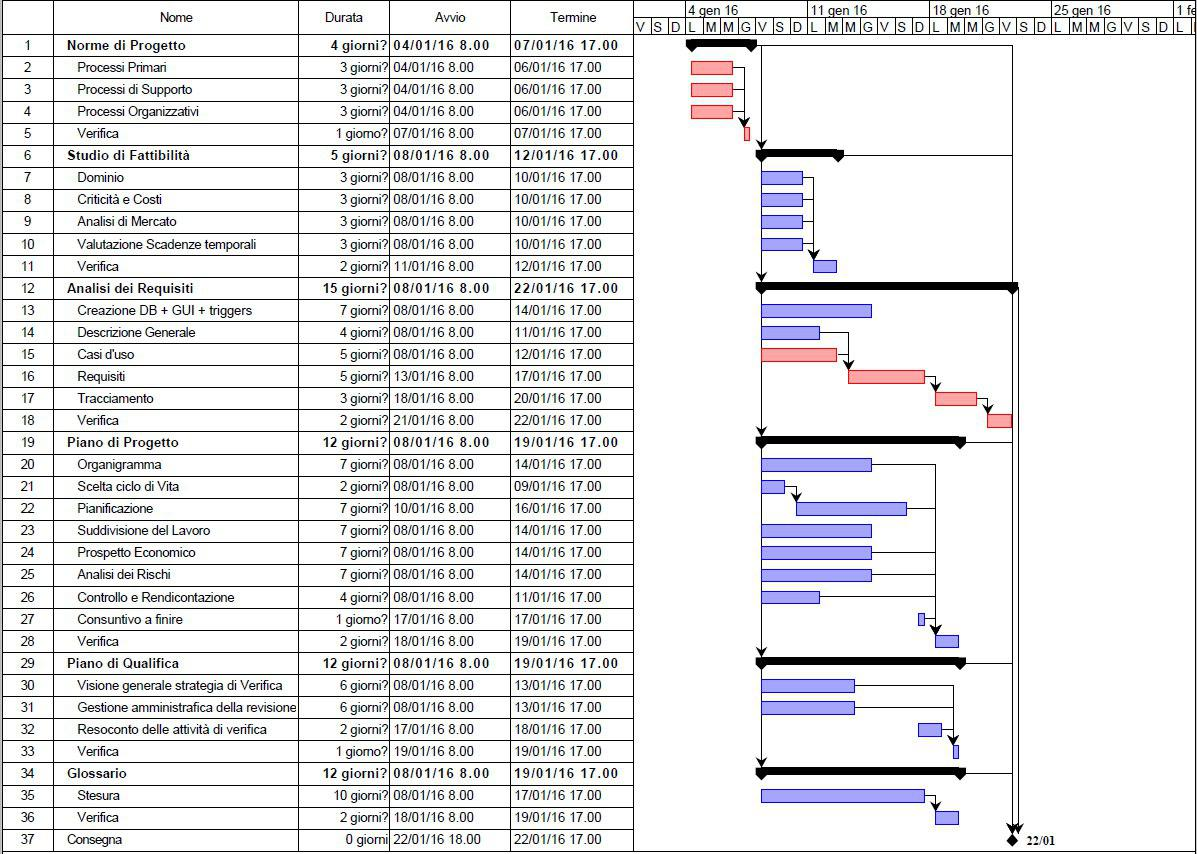
\includegraphics[scale=0.4]{GanttAnalisi}
					\caption{Gantt attività - fase di Analisi.}
				\end{figure}
			\subsection{WBS attività}
				%Image
				\begin{figure}[H]
					\centering
					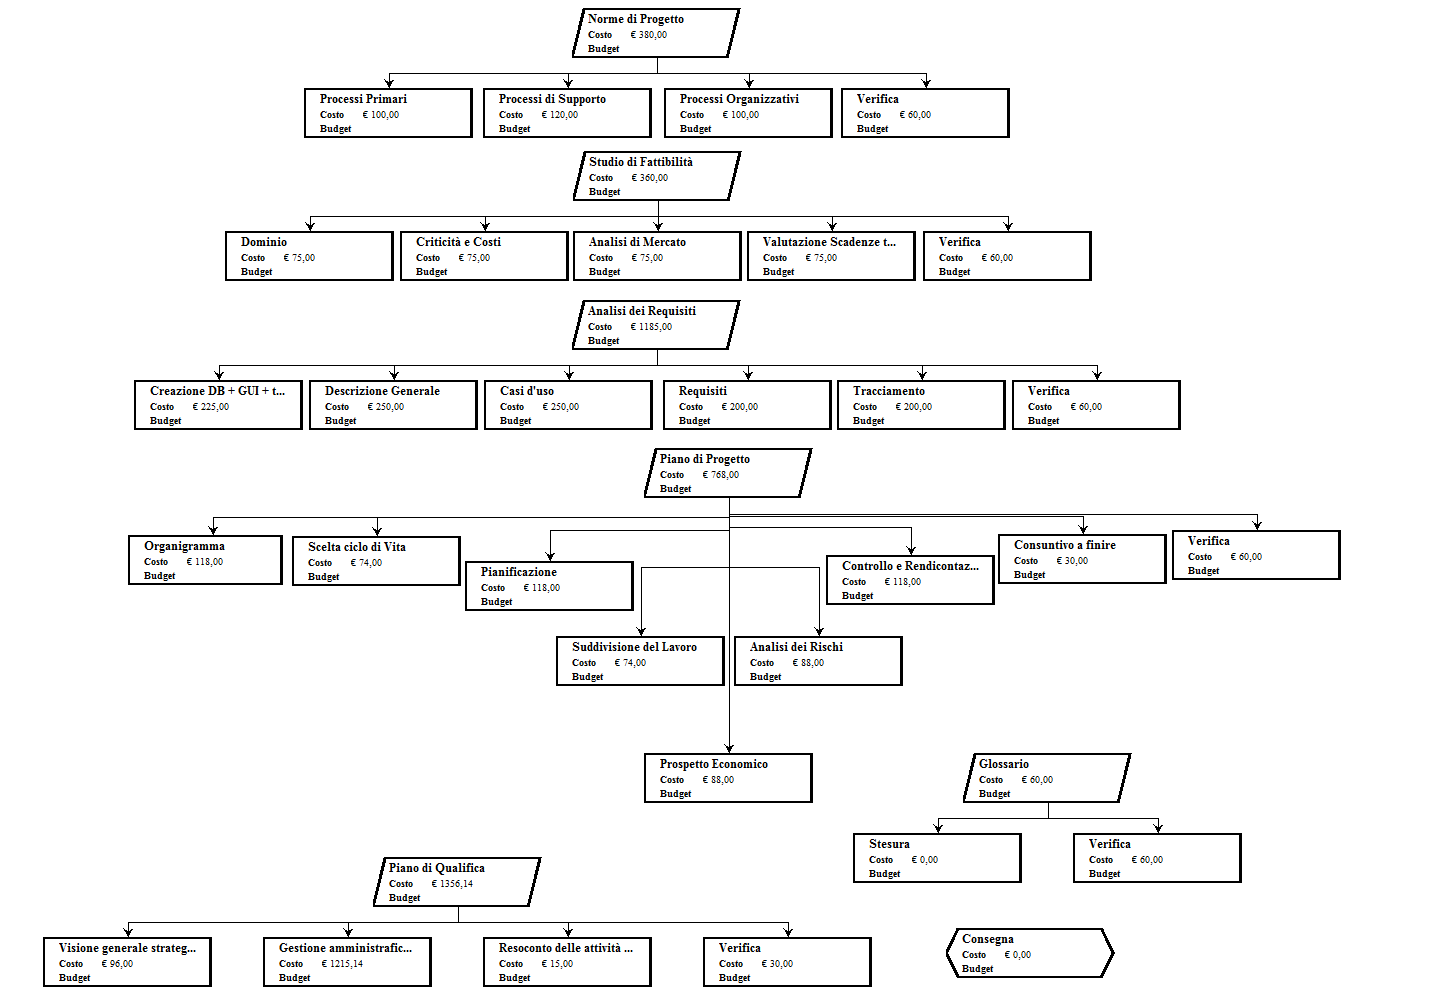
\includegraphics[scale=0.5]{WBSAnalisi}
					\caption{Work Breakdown Structure - fase di Analisi.}
				\end{figure}
			\subsection{Ripartizione ore}
				%Image
				\begin{figure}[H]
					\centering
					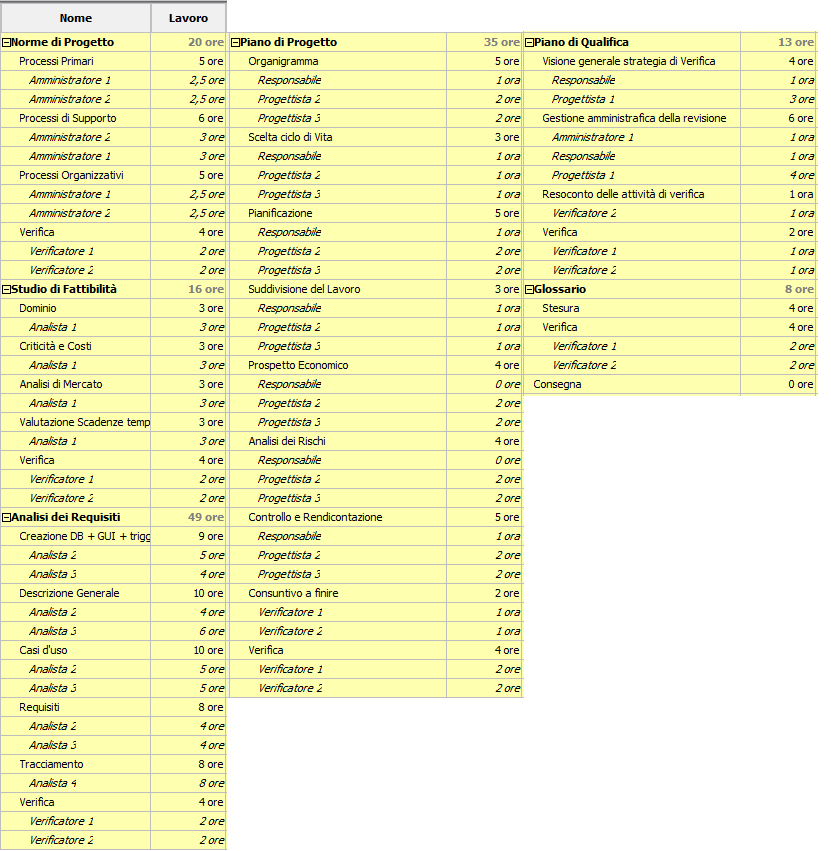
\includegraphics[scale=0.6]{ROAnalisi}
					\caption{Ripartizione ore - fase di Analisi.}
				\end{figure}

		\section{Analisi di dettaglio}
			\textbf{Periodo:} da 2016-01-23 a 2016-03-01 \\
			Questa fase ha inizio subito dopo la consegna dei documenti alla \emph{Revisione dei requisiti}, la
			prima scadenza che il gruppo intende rispettare; con l'inizio della macro-fase successiva, ovvero la 
			progettazione architetturale.
			Questo periodo viene usato per migliorare i requisiti proposti e per aggiornare il documento di 
			\emph{Analisi dei requisiti}. 
			Le attività sono le stesse della fase di \emph{Analisi}, escluso lo \emph{Studio di fattibilità}. 
			In questa macro-fase i ruoli maggiormente coinvolti sono: \emph{Responsabile}, \emph{Amministratore} 
			e \emph{Analista}.
			\subsection{Gantt attività}
				%Image
				\begin{figure}[H]
					\centering
					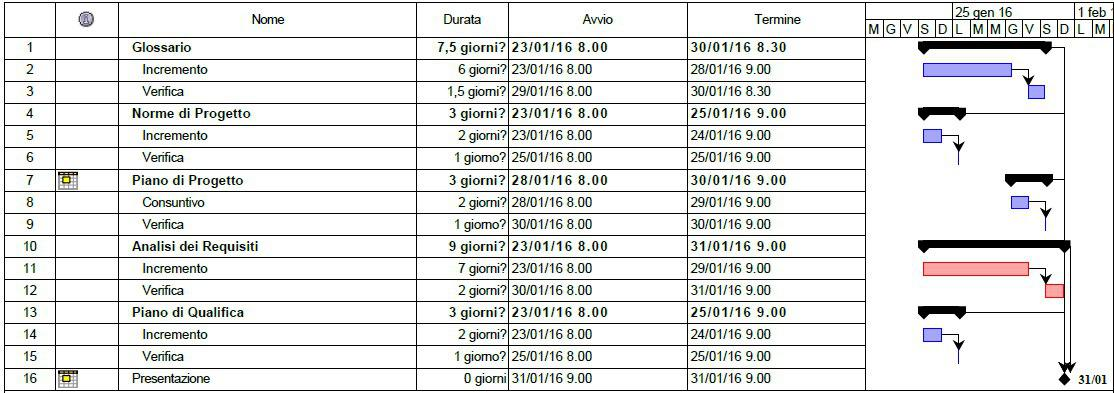
\includegraphics[scale=0.5]{GanttDettaglio}
					\caption{Gantt attività - fase di Analisi di dettaglio.}
				\end{figure}
			\subsection{WBS attività}
				%Image
				\begin{figure}[H]
					\centering
					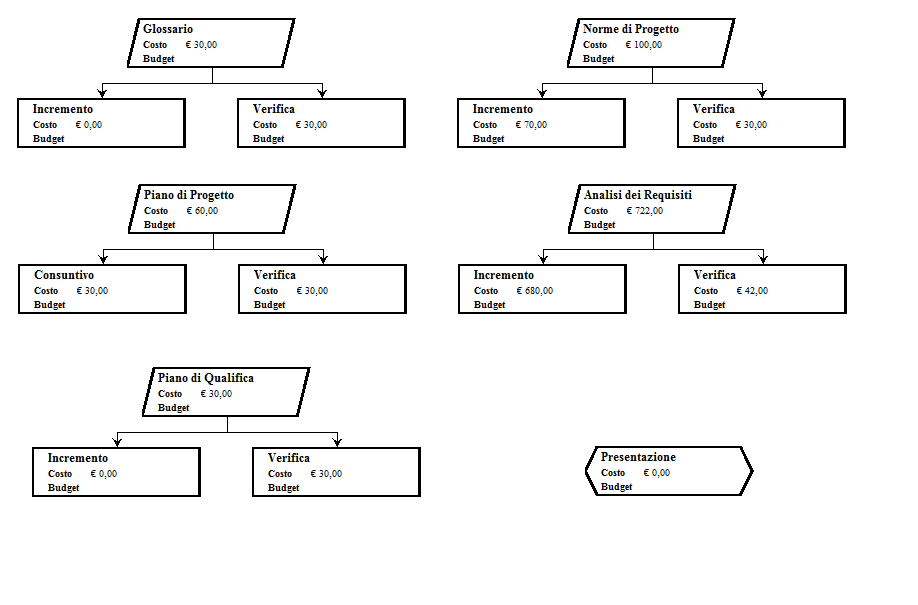
\includegraphics[scale=0.5]{WBSDettaglio}
					\caption{Work Breakdown Structure - fase di Analisi.}
				\end{figure}
			\subsection{Ripartizione ore}
				%Image
				\begin{figure}[H]
					\centering
					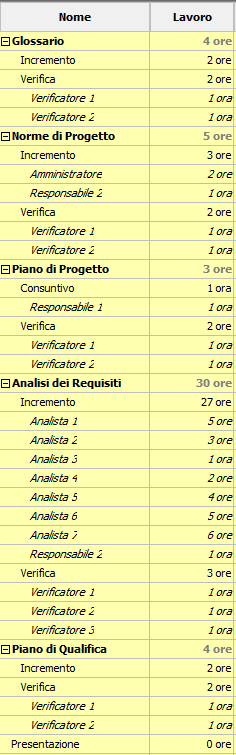
\includegraphics[scale=0.6]{RODettaglio}
					\caption{Ripartizione ore - fase di Analisi di dettaglio.}
				\end{figure}
		\section{Progettazione architetturale}
			\textbf{Periodo:} da 2016-02-01 a 2016-03-20 \\
			Questa macro-fase inizia al termine dell'\emph{Analisi di dettaglio} e termina con la conclusione 
			della progettazione ad alto livello del progetto, prima della seconda scadenza. In questa fase viene 
			descritta la struttura logica ad alto livello del prodotto, mentre il suo stato definitivo viene 
			descritto nella macro-fase successiva. \\
			Le attività in questa fase sono:
			\begin{itemize}
				\item \textbf{Specifica tecnica:} i progettisti del gruppo esporranno le scelte progettuali ad alto 
				livello che il prodotto dovrà assicurare. Verranno descritti i design pattern designati per lo sviluppo, 
				l'architettura generale del software, il tracciamento dei requisiti e i principali flussi di controllo;
				\item \textbf{Incremento e verifica:} tutti i documenti in questa macro-fase verranno aggiornati in base 
				al risultato della \emph{Revisione dei requisiti}.
			\end{itemize}
			In questa fase i ruoli principalmente coinvolti sono: \emph{Responsabile}, \emph{Amministratore},
			\emph{Progettista}, \emph{Verificatore} e  \emph{Analista}.

			\subsection{Gantt attività}
				%Image
				\begin{figure}[H]
					\centering
					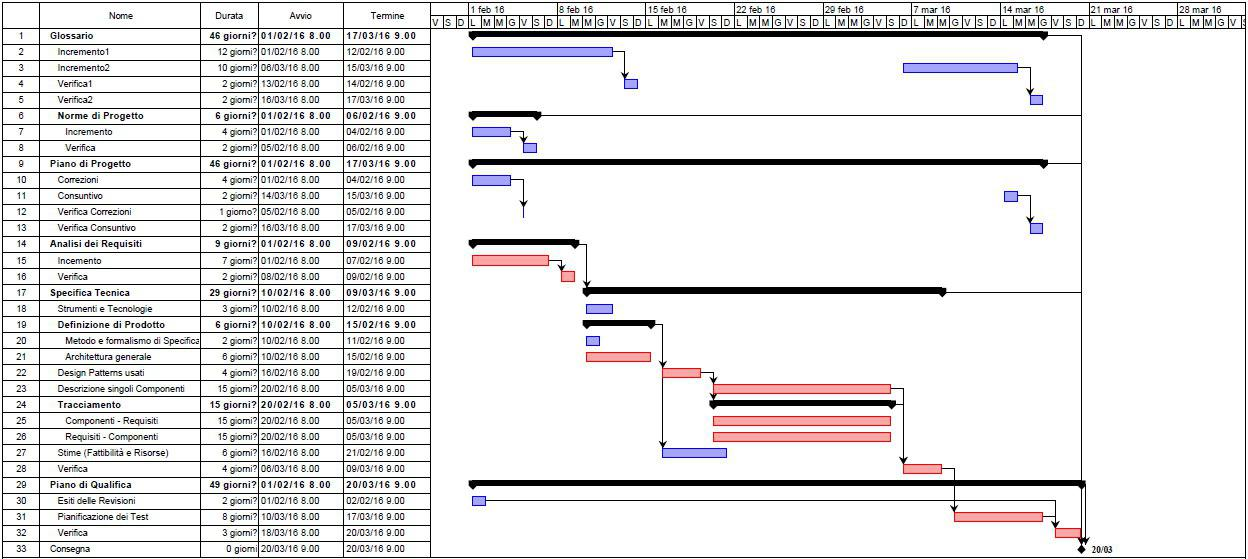
\includegraphics[scale=0.4]{GanttProgettazione}
					\caption{Gantt attività - fase di Progettazione architetturale.}
				\end{figure}
			\subsection{WBS attività}
				%Image
				\begin{figure}[H]
					\centering
					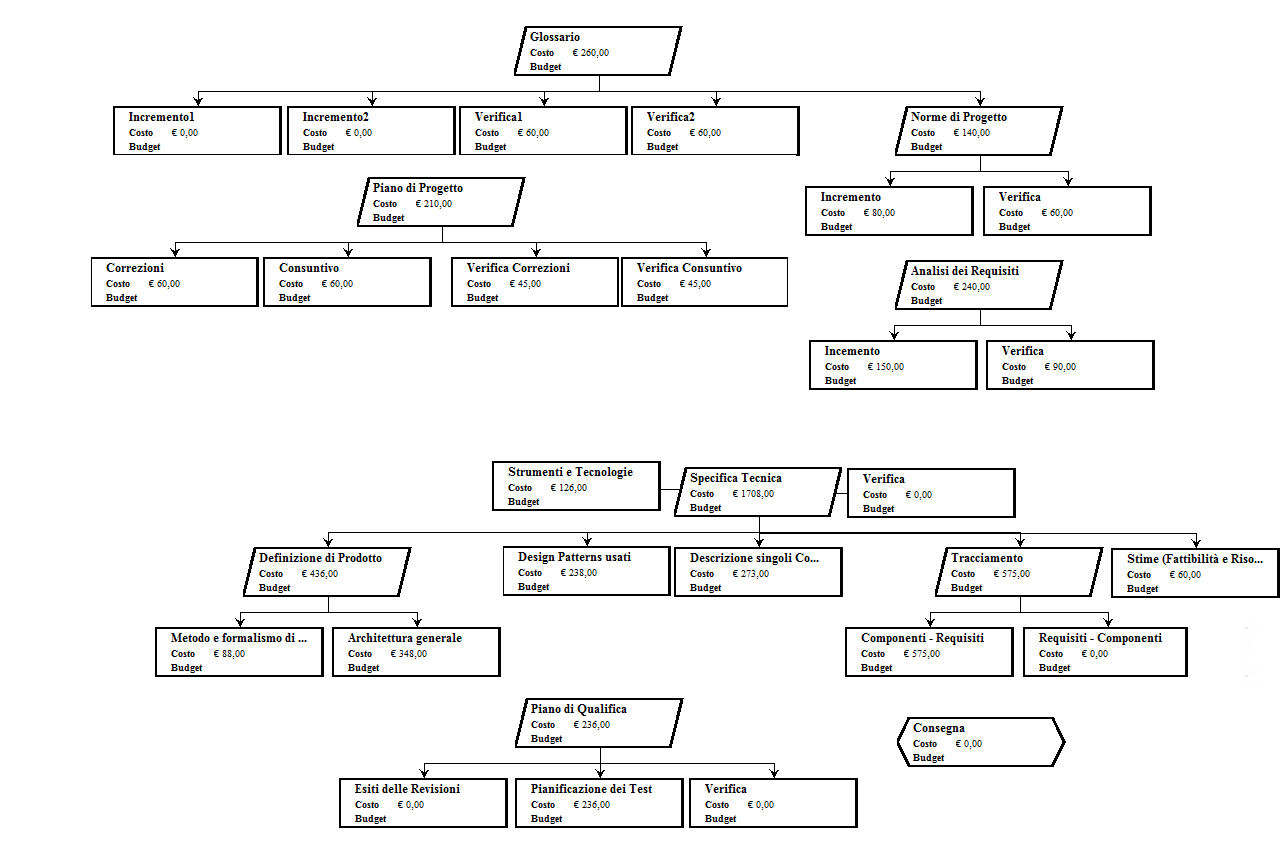
\includegraphics[scale=0.3]{WBSProgettazione}
					\caption{Work Breakdown Structure - fase di Analisi.}
				\end{figure}
			\subsection{Ripartizione ore}
				%Image
				\begin{figure}[H]
					\centering
					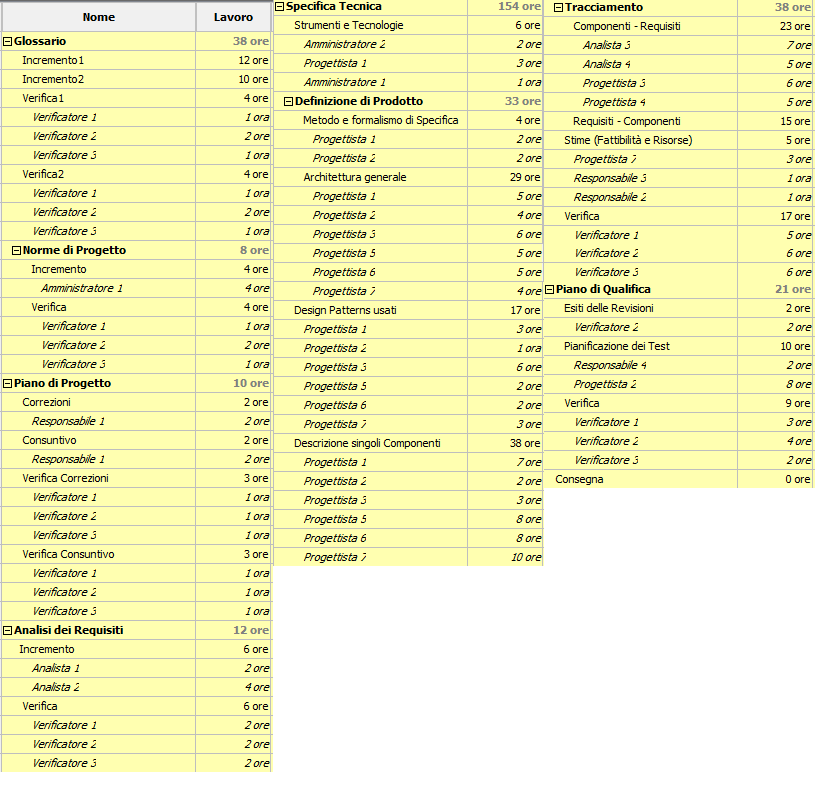
\includegraphics[scale=0.6]{ROProgettazione}
					\caption{Ripartizione ore - fase di Progettazione architetturale.}
				\end{figure}
				
		\section{Progettazione di dettaglio e codifica}
			\textbf{Periodo:} da 2016-03-21 a 2016-05-23 \\
			Questa macro-fase ha inizio immediatamente dopo la fine della progettazione di alto livello, attraversa la seconda 
			scadenza che il gruppo intende rispettare, la \emph{Revisione di progetto} ed ha il compito di descrivere nel dettaglio 
			l'architettura del prodotto, e la sua realizzazione. La scadenza di questa fase è definita dalla 
			\emph{Revisione di qualifica}. \\Le attività principali di questa fase sono:
			\begin{itemize}
				\item \textbf{Definizione di Prodotto:} in questo definita in modo approfondito la struttura e le relazioni 
				dei vari componenti del prodotto, basandosi sul documento di \emph{Specifica tecnica}; 
				\item \textbf{Codifica:} in questa fase inizia lo sviluppo del codice del prodotto da parte dei programmatori, 
				tenuti a seguire quanto specificato nel documento \emph{Definizione di prodotto};
				\item \textbf{Manuali utente:} questi documenti avranno lo scopo di illustrare delle linee guida per l'utilizzo 
				del sistema da parte degli utenti;
				\item \textbf{Incremento e verifica:} tutti i documenti verranno aggiornati per la presentazione alla 
				\emph{Revisione di qualifica}.
			\end{itemize}
			In questa fase i ruoli principalmente coinvolti sono: \emph{Responsabile}, \emph{Amministratore},
			\emph{Progettista} e \emph{Verificatore}.

			\subsection{Gantt attività}
				%Image
				\begin{figure}[H]
					\centering
					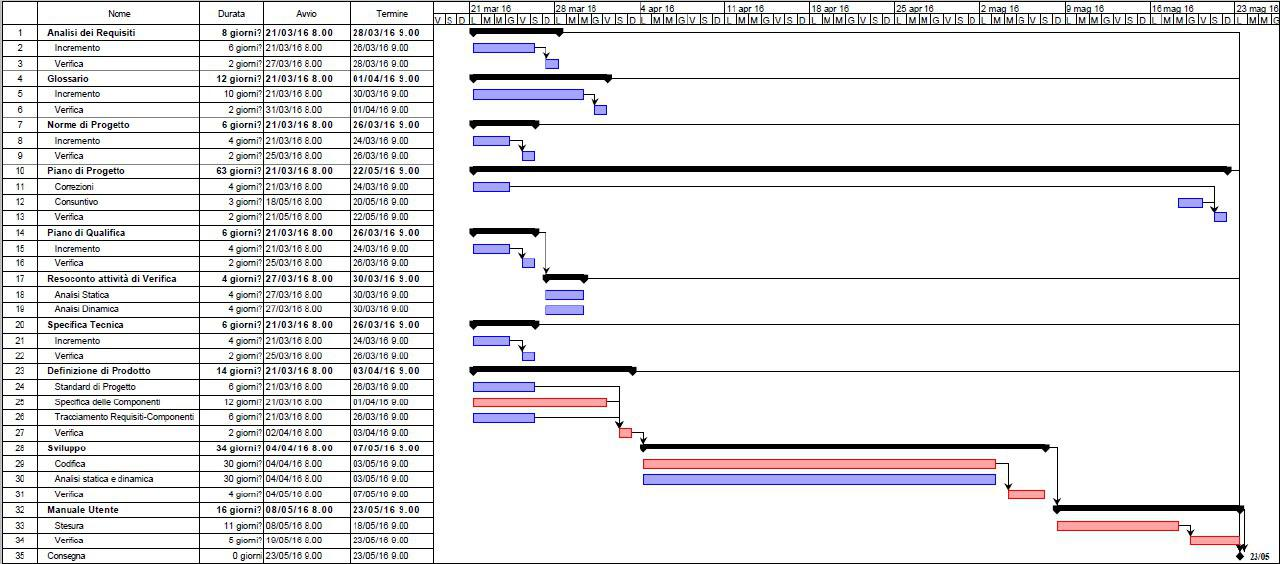
\includegraphics[scale=0.4]{GanttCodifica}
					\caption{Gantt attività - fase di Progettazione di dettaglio e codifica.}
				\end{figure}
			\subsection{WBS attività}
				%Image
				\begin{figure}[H]
					\centering
					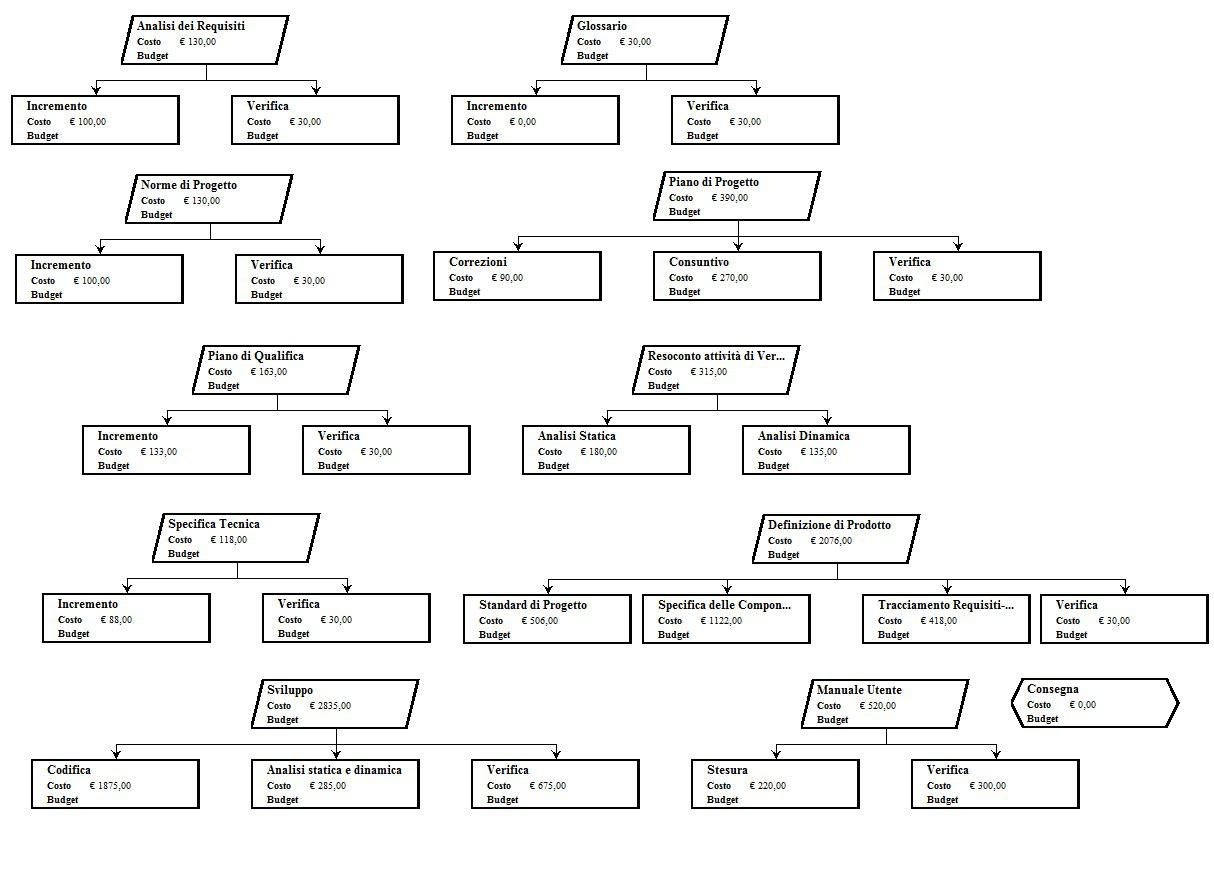
\includegraphics[scale=0.3]{WBSCodifica}
					\caption{Work Breakdown Structure - fase di Progettazione di dettaglio e codifica.}
				\end{figure}
			\subsection{Ripartizione ore}
				%Image
				\begin{figure}[H]
					\centering
					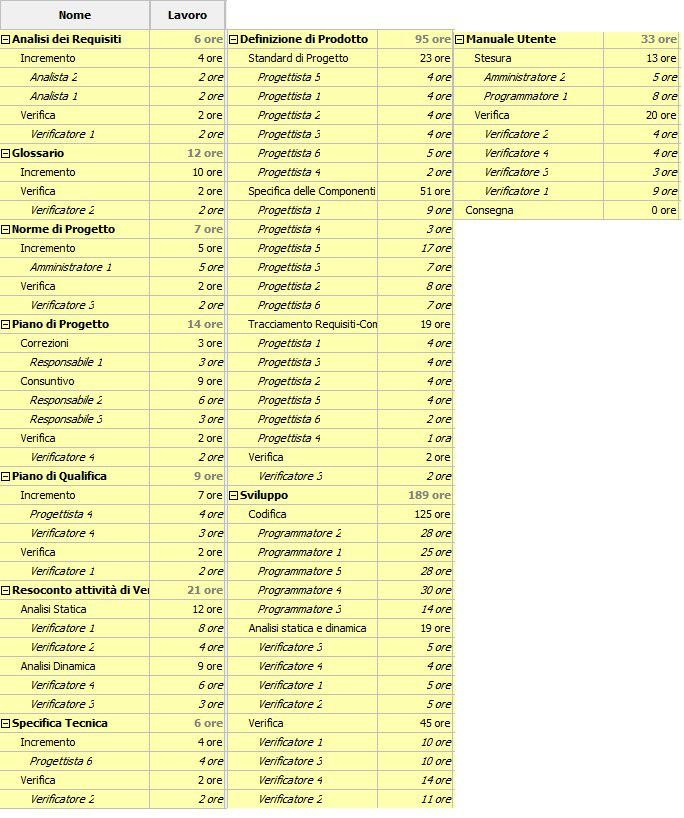
\includegraphics[scale=0.6]{ROCodifica}
					\caption{Ripartizione ore - fase di Progettazione di dettaglio e codifica.}
				\end{figure}
		\section{Verifica e validazione}
			\textbf{Periodo:} da 2016-05-24 a 2016-06-19 \\
			Ultima macro-fase del progetto, in questa fase, successiva alla \emph{Revisione di qualifica} il gruppo 
			intende effettuare gli ultimi test di verifica, e la validazione del prodotto. Il termine ultimo, di questa 
			fase, ma anche del progetto, è la \emph{Revisione di accettazione}. \\ Le attività coinvolte sono:
			\begin{itemize}
				\item \textbf{Ambiente di validazione e collaudo del sistema:} in questa attività il prodotto verrà 
				convalidato, verrà quindi dimostrato che è conforme alle specifiche e soddisfa le richieste del committente;
				\item \textbf{Incremento e verifica:} tutti i documenti verranno aggiornati in base al risultato della 
				\emph{Revisione di qualifica} e preparati per la \emph{Revisione di accettazione}.
			\end{itemize}
			\subsection{Gantt attività}
				%Image
				\begin{figure}[H]
					\centering
					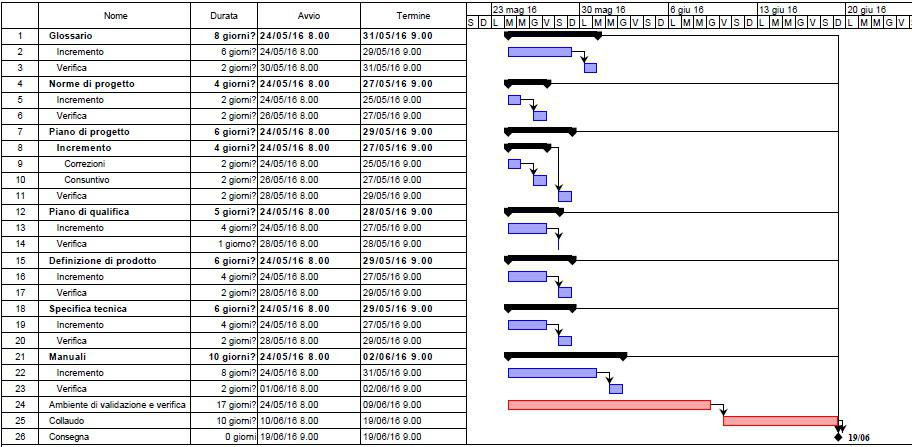
\includegraphics[scale=0.4]{GanttValidazione}
					\caption{Gantt attività - fase di Verifica e validazione.}
				\end{figure}
			\subsection{WBS attività}
				%Image
				\begin{figure}[H]
					\centering
					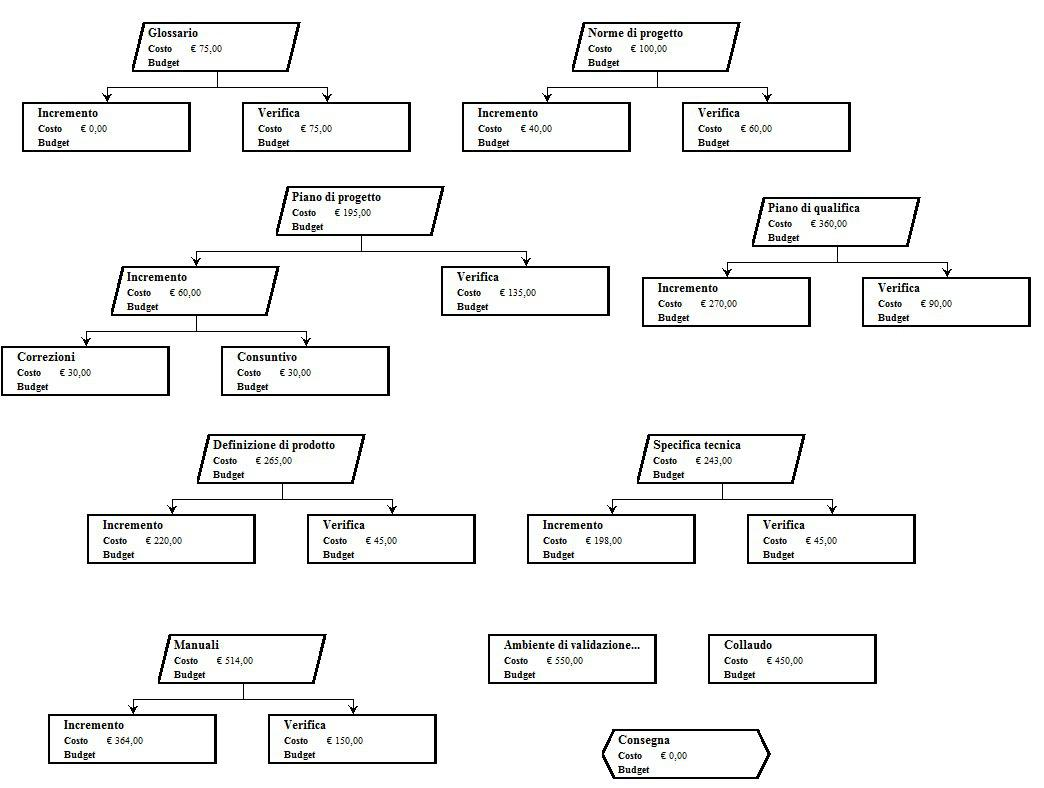
\includegraphics[scale=0.5]{WBSValidazione}
					\caption{Work Breakdown Structure - fase di Verifica e validazione.}
				\end{figure}
			\subsection{Ripartizione ore}
				%Image
				\begin{figure}[H]
					\centering
					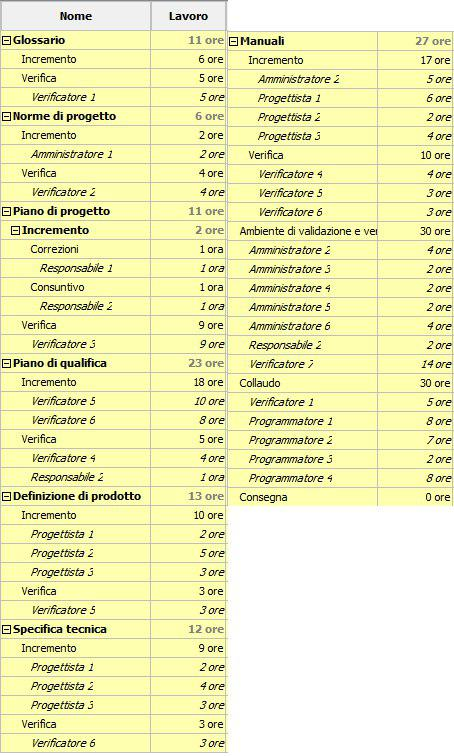
\includegraphics[scale=0.6]{ROValidazione}
					\caption{Ripartizione ore - fase di Verifica e validazione.}
				\end{figure}

	\mychapter{3}{Suddivisione del lavoro}
		Ogni membro del gruppo, dovrà, durante tutta la durata del progetto, ricoprire almeno una volta ciascuno dei
		ruoli descritti nell'appendice, sezione A.5. Durante ogni fase ogni membro può ricoprire
		più ruoli contemporaneamente, a patto che non si verifichino dei conflitti di interesse tra i ruoli ricoperti. 
		Un membro del gruppo non può verificare il suo stesso lavoro.
		\section{Dettaglio delle fasi}
			\subsection{Analisi}
				Nella fase di \emph{Analisi} ciascun componente dovrà ricoprire i seguenti ruoli:
				\begin{table}[H]
					\begin{tabularx}{\textwidth}{ r t t t t t t | >{\centering\arraybackslash}t } 
						\rowcolor{orange!85}& \multicolumn{6}{c}{Ore per ruoli} &  \\
						\rowcolor{orange!85}Nominativo & Re & Am & An & Pt & Ve & Pr & Totali\\ 
						\noalign{\hrule height 1.5pt}
						\multicolumn{1}{r|}{Biggeri Mattia} & & & & 7 & 13 & & 20\\
						\multicolumn{1}{r|}{Bonato Paolo} & & & 18 & & & & 18\\ 
						\multicolumn{1}{r|}{Bortolazzo Matteo} & & & 19 & & & & 19\\ 
						\multicolumn{1}{r|}{Maino Elia} & & 8 & 12 & & & & 20\\
						\multicolumn{1}{r|}{Nicoletti Luca} & & 8 & & 12 & & & 20\\
						\multicolumn{1}{r|}{Padovan Tommaso} & 7 & & & 12 & & & 19\\
						\multicolumn{1}{r|}{Tommasin Davide} & & & 8 & & 12 & & 20\\
						\noalign{\hrule height 1.5pt}						
					\end{tabularx}
				\caption{Ripartizione ore - fase di Analisi. } 
				\label{TRAnalisi}
				\end{table}
				I valori sono rappresentati nel grafico, per semplificare la visualizzazione di quante ore ciascun membro 
				abbia dedicato ad un determinato ruolo.
				%Image
				\begin{figure}[H]
					\centering
					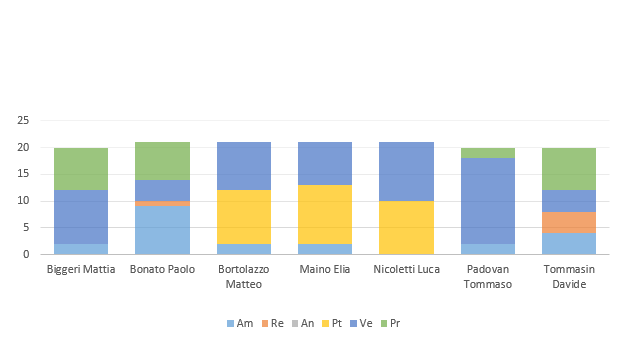
\includegraphics[scale=0.8]{BCAnalisi.png}
					\caption{Ore per componente, fase di Analisi.}
				\end{figure}
			\subsection{Analisi di dettaglio}
				Nella fase di \emph{Analisi di dettaglio} ciascun componente dovrà ricoprire i seguenti ruoli:
				\begin{table}[H]
					\begin{tabularx}{\textwidth}{ r t t t t t t | >{\centering\arraybackslash}t } 
						\rowcolor{orange!85}& \multicolumn{6}{c}{Ore per ruoli} &  \\
						\rowcolor{orange!85}Nominativo & Re & Am & An & Pt & Ve & Pr & Totali\\ 
						\noalign{\hrule height 1.5pt}
						\multicolumn{1}{r|}{Biggeri Mattia} & & & 5 & & & & 5\\
						\multicolumn{1}{r|}{Bonato Paolo} & 2 & & 3 & & & & 5\\ 
						\multicolumn{1}{r|}{Bortolazzo Matteo} & & & 1 & & 5 & & 6\\ 
						\multicolumn{1}{r|}{Maino Elia} & & & & 2 & 5 & & 7\\
						\multicolumn{1}{r|}{Nicoletti Luca} & 2 & & 4 & & 1 & & 7\\
						\multicolumn{1}{r|}{Padovan Tommaso} & 1 & & 5 & & & & 6\\
						\multicolumn{1}{r|}{Tommasin Davide} & & & 6 & & & & 6\\
						\noalign{\hrule height 1.5pt}						
					\end{tabularx}
					\caption{Ripartizione ore - fase di Analisi di dettaglio. } 
					\label{TRDettaglio}
				\end{table}
				I valori sono rappresentati nel grafico, per semplificare la visualizzazione di quante ore ciascun membro 
				abbia dedicato ad un determinato ruolo.
				%Image
				\begin{figure}[H]
					\centering
					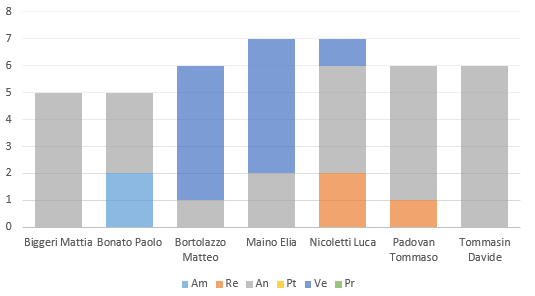
\includegraphics[scale=0.9]{BCDettaglio.png}
					\caption{Ore per componente, fase di Analisi di dettaglio.}
				\end{figure}
			\subsection{Progettazione architetturale}
				Nella fase di \emph{Progettazione architetturale} ciascun componente dovrà ricoprire i seguenti ruoli:
				\begin{table}[H]
					\begin{tabularx}{\textwidth}{ r t t t t t t | >{\centering\arraybackslash}t } 
						\rowcolor{orange!85}& \multicolumn{6}{c}{Ore per ruoli} &  \\
						\rowcolor{orange!85}Nominativo & Re & Am & An & Pt & Ve & Pr & Totali\\ 
						\noalign{\hrule height 1.5pt}
						\multicolumn{1}{r|}{Biggeri Mattia} & 4 & & 20 & & & & 24\\
						\multicolumn{1}{r|}{Bonato Paolo} & & & 2 & 17 & 15 & & 34\\ 
						\multicolumn{1}{r|}{Bortolazzo Matteo} & 1 & & 4 & 22 & & & 27\\ 
						\multicolumn{1}{r|}{Maino Elia} & 1 & & 5 & 22 & & & 28\\
						\multicolumn{1}{r|}{Nicoletti Luca} & 2 & & 15 & 15 & & & 32\\
						\multicolumn{1}{r|}{Padovan Tommaso} & & 5 & 7 & 15 & & & 27\\
						\multicolumn{1}{r|}{Tommasin Davide} & & 2 & 3 & 20 & & & 25\\
						\noalign{\hrule height 1.5pt}						
					\end{tabularx}
					\caption{Ripartizione ore - fase di Progettazione architetturale. } 
					\label{TRProgettazione}
				\end{table}
				I valori sono rappresentati nel grafico, per semplificare la visualizzazione di quante ore ciascun membro 
				abbia dedicato ad un determinato ruolo.
				%Image
				\begin{figure}[H]
					\centering
					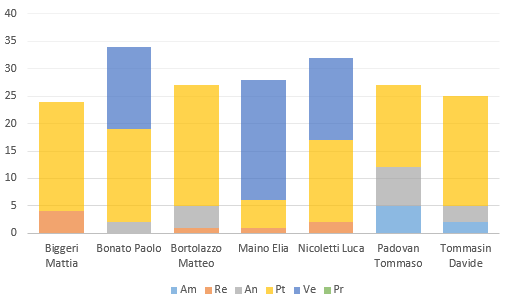
\includegraphics[scale=0.9]{BCProgettazione.png}
					\caption{Ore per componente, fase di Progettazione architetturale.}
				\end{figure}
			\subsection{Progettazione di dettaglio e codifica}
				Nella fase di \emph{Progettazione di dettaglio e codifica} ciascun componente dovrà ricoprire i seguenti ruoli:
				\begin{table}[H]
					\begin{tabularx}{\textwidth}{ r t t t t t t | >{\centering\arraybackslash}t } 
						\rowcolor{orange!85}& \multicolumn{6}{c}{Ore per ruoli} &  \\
						\rowcolor{orange!85}Nominativo & Re & Am & An & Pt & Ve & Pr & Totali\\ 
						\noalign{\hrule height 1.5pt}
						\multicolumn{1}{r|}{Biggeri Mattia} & & 5 & & 17 & & 33 & 55\\
						\multicolumn{1}{r|}{Bonato Paolo} & 3 & & & 16 & 36 & & 55\\ 
						\multicolumn{1}{r|}{Bortolazzo Matteo} & 6 & 5 & & 15 & & 28 & 54\\ 
						\multicolumn{1}{r|}{Maino Elia} & 3 & & & 10 & 28 & 14 & 55\\
						\multicolumn{1}{r|}{Nicoletti Luca} & & & & 25 & & 30 & 55\\
						\multicolumn{1}{r|}{Padovan Tommaso} & & & 2 & & 25 & 28 & 55\\
						\multicolumn{1}{r|}{Tommasin Davide} & & & 2 & 18 & 33 & & 53\\
						\noalign{\hrule height 1.5pt}						
					\end{tabularx}
					\caption{Ripartizione ore - fase di Progettazione di dettaglio e codifica. } 
					\label{TRCodifica}
				\end{table}
				I valori sono rappresentati nel grafico, per semplificare la visualizzazione di quante ore ciascun membro 
				abbia dedicato ad un determinato ruolo.
				%Image
				\begin{figure}[H]
					\centering
					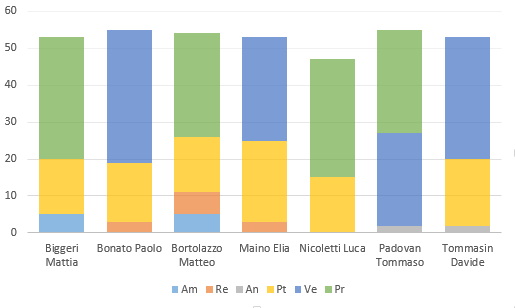
\includegraphics[scale=0.9]{BCCodifica.png}
					\caption{Ore per componente, fase di Progettazione di dettaglio e codifica.}
				\end{figure}
			\subsection{Verifica e validazione}
				Nella fase di \emph{Verifica e validazione} ciascun componente dovrà ricoprire i seguenti ruoli:
				\begin{table}[H]
					\begin{tabularx}{\textwidth}{ r t t t t t t | >{\centering\arraybackslash}t } 
						\rowcolor{orange!85}& \multicolumn{6}{c}{Ore per ruoli} &  \\
						\rowcolor{orange!85}Nominativo & Re & Am & An & Pt & Ve & Pr & Totali\\ 
						\noalign{\hrule height 1.5pt}
						\multicolumn{1}{r|}{Biggeri Mattia} & & 2 & & & 10 & 8 & 20\\
						\multicolumn{1}{r|}{Bonato Paolo} & 1 & 9 & & & 4 & 7 & 21\\ 
						\multicolumn{1}{r|}{Bortolazzo Matteo} & & 2 & & 10 & 9 & & 21\\ 
						\multicolumn{1}{r|}{Maino Elia} & & 2 & & 11 & 8 & & 21\\
						\multicolumn{1}{r|}{Nicoletti Luca} & & & & 10 & 11 & & 21\\
						\multicolumn{1}{r|}{Padovan Tommaso} & & 2 & & & 16 & 2 & 20\\
						\multicolumn{1}{r|}{Tommasin Davide} & 4 & 4 & & & 4 & 8 & 20\\
						\noalign{\hrule height 1.5pt}						
					\end{tabularx}
					\caption{Ripartizione ore - fase di Verifica e validazione. } 
					\label{TRVeV}
				\end{table}
				I valori sono rappresentati nel grafico, per semplificare la visualizzazione di quante ore ciascun membro 
				abbia dedicato ad un determinato ruolo.
				%Image
				\begin{figure}[H]
					\centering
					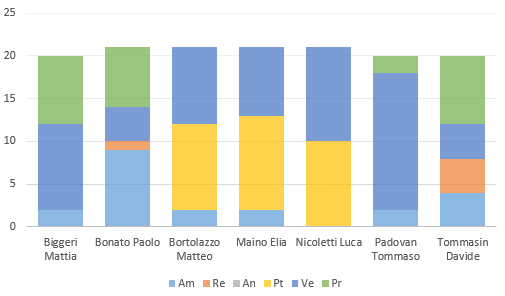
\includegraphics[scale=0.9]{BCValidazione.png}
					\caption{Ore per componente, fase di Verifica e validazione.}
				\end{figure}
		\section{Totali}
			\subsection{Totale ore con investimento}
				Contando anche le ore di investimento, le ore che ciascun membro dedicherà 
				allo svolgimento del progetto saranno le seguenti:
				\begin{table}[H]
					\begin{tabularx}{\textwidth}{ r t t t t t t | >{\centering\arraybackslash}t } 
						\rowcolor{orange!85}& \multicolumn{6}{c}{Ore per ruoli} &  \\
						\rowcolor{orange!85}Nominativo & Re & Am & An & Pt & Ve & Pr & Totali\\ 
						\noalign{\hrule height 1.5pt}
						\multicolumn{1}{r|}{Biggeri Mattia} & 4 & 7 & 5 & 44 & 23 & 41 & 124\\
						\multicolumn{1}{r|}{Bonato Paolo} & 4 & 11 & 23 & 33 & 55 & 7 & 133\\ 
						\multicolumn{1}{r|}{Bortolazzo Matteo} & 7 & 7 & 24 & 47 & 14 & 28 & 127\\ 
						\multicolumn{1}{r|}{Maino Elia} & 4 & 10 & 14 & 26 & 63 & 14 & 131\\
						\multicolumn{1}{r|}{Nicoletti Luca} & 4 & 8 & 4 & 62 & 27 & 30 & 135\\
						\multicolumn{1}{r|}{Padovan Tommaso} & 8 & 7 & 14 & 27 & 41 & 30 & 127\\
						\multicolumn{1}{r|}{Tommasin Davide} & 4 & 6 & 11 & 38 & 49 & 8 & 116\\
						\noalign{\hrule height 1.5pt}						
					\end{tabularx}
					\caption{Ripartizione ore - totale con investimento. } 
					\label{TRTotale}
				\end{table}
				I valori sono rappresentati nel grafico, per semplificare la visualizzazione di quante ore ciascun membro 
				abbia dedicato ad un determinato ruolo.
				%Image
				\begin{figure}[H]
					\centering
					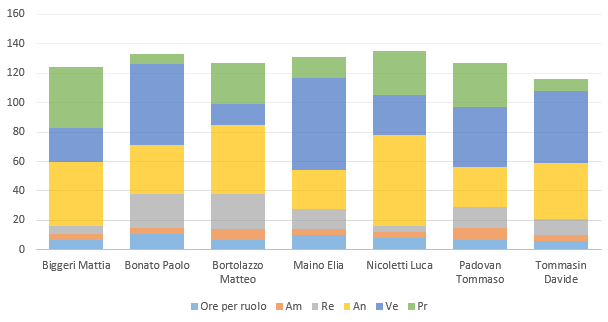
\includegraphics[scale=0.9]{BCTotali.png}
					\caption{Ore per componente, fase di Verifica e validazione.}
				\end{figure}
			\subsection{Totale ore rendicontate}
				Le ore rendicontate, sono minori rispetto alle ore totali, in quanto non sono a 
				carico del committente le fasi di \emph{Analisi dei requisiti} e l'
				\emph{Analisi di dettaglio}.
				\begin{table}[H]
					\begin{tabularx}{\textwidth}{ r t t t t t t | >{\centering\arraybackslash}t } 
						\rowcolor{orange!85}& \multicolumn{6}{c}{Ore per ruoli} &  \\
						\rowcolor{orange!85}Nominativo & Re & Am & An & Pt & Ve & Pr & Totali\\ 
						\noalign{\hrule height 1.5pt}
						\multicolumn{1}{r|}{Biggeri Mattia} & 4 & 7 & & 37 & 10 & 41 & 99\\
						\multicolumn{1}{r|}{Bonato Paolo} & 4 & 9 & 2 & 33 & 55 & 7 & 110\\ 
						\multicolumn{1}{r|}{Bortolazzo Matteo} & 7 & 7 & 4 & 47 & 9 & 28 & 102\\ 
						\multicolumn{1}{r|}{Maino Elia} & 4 & 2 & & 26 & 58 & 14 & 104\\
						\multicolumn{1}{r|}{Nicoletti Luca} & 2 & & & 50 & 26 & 30 & 108\\
						\multicolumn{1}{r|}{Padovan Tommaso} & & 7 & 9 & 15 & 41 & 30 & 102\\
						\multicolumn{1}{r|}{Tommasin Davide} & 4 & 6 & 5 & 38 & 37 & 8 & 98\\
						\noalign{\hrule height 1.5pt}						
					\end{tabularx}
					\caption{Ripartizione ore - totale rendicontate. } 
					\label{TRRendicontate}
				\end{table}
				I valori sono rappresentati nel grafico, per semplificare la visualizzazione di quante ore ciascun membro 
				abbia dedicato ad un determinato ruolo.
				%Image
				\begin{figure}[H]
					\centering
					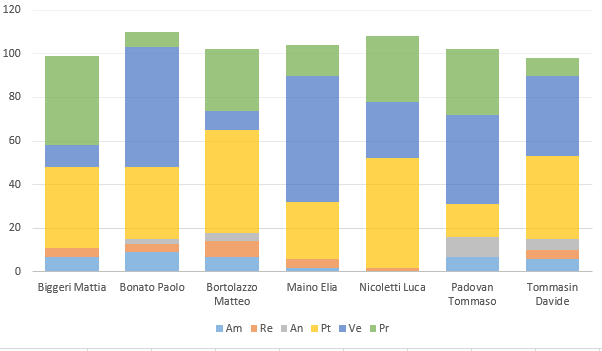
\includegraphics[scale=0.9]{BCRendicontate.png}
					\caption{Ore per componente, fase di Verifica e validazione.}
				\end{figure}
	\mychapter{4}{Prospetto economico}
		Per ciascuna fase del progetto, in questa sezione vengono presentate le ore preventivate di impiego per tutti i 
		ruoli coinvolti. Si ricorda che le fasi di \emph{Analisi dei requisiti} e \emph{Analisi di dettaglio} non sono 
		a carico del committente e quindi non saranno considerate nel calcolo delle ore preventivate.
		\section{Analisi}
			Nelle fase di \emph{Analisi}, le ore per ciascun ruolo sono state suddivise in questo modo:
			\begin{table}[H]
				\begin{tabularx}{\textwidth}{Y Y Y}
					\noalign{\hrule height 1.5pt}
					\rowcolor{orange!85}Ruolo & Ore & Costo \\
					\noalign{\hrule height 1.5pt}
					Responsabile & 7 & 140 \\
					Amministratore & 16 & 480 \\
					Analista & 57 & 1425\\
					Progettista & 31 & 682\\
					Verificatore & 25 & 375\\
					Programmatore & 0 & 0 \\
					\noalign{\hrule height 0.5pt}
					\textbf{Totali} & 136 & 3012 \\
					\noalign{\hrule height 1.5pt}
				\end{tabularx}
				\caption{Costo ore - fase di Analisi. } 
				\label{TCAnalisi}
			\end{table}
			I seguenti grafici mostrano come ogni ruolo e il rispettivo costo abbiano influito sul calcolo del totale 
			costo della fase di \emph{Analisi}.
			%Image
			\begin{figure}[H]
				\centering
				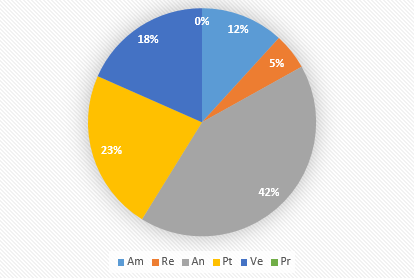
\includegraphics[scale=0.7]{PCAnalisi}
				\caption{Ore per ruolo, fase di Analisi.}
			\end{figure}
			%Image
			\begin{figure}[H]
				\centering
				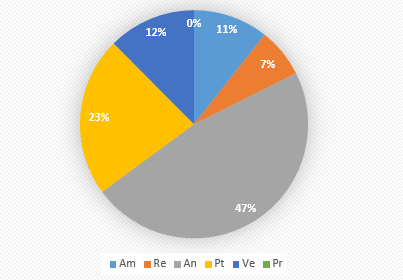
\includegraphics[scale=0.7]{PCCostiAnalisi}
				\caption{Costi per ruolo, fase di Analisi.}
			\end{figure}
		\section{Analisi di dettaglio}
			Nelle fase di \emph{Analisi di dettaglio}, le ore per ciascun ruolo sono state suddivise in questo modo:
			\begin{table}[H]
				\begin{tabularx}{\textwidth}{Y Y Y}
					\noalign{\hrule height 1.5pt}
					\rowcolor{orange!85}Ruolo & Ore & Costo \\
					\noalign{\hrule height 1.5pt}
					Responsabile & 3 & 90 \\
					Amministratore & 2 & 40 \\
					Analista & 26 & 650\\
					Progettista & 0 & 0\\
					Verificatore & 11 & 165\\
					Programmatore & 0 & 0 \\
					\noalign{\hrule height 0.5pt}
					\textbf{Totali} & 42 & 945 \\
					\noalign{\hrule height 1.5pt}
				\end{tabularx}
				\caption{Costo ore - fase di Analisi di dettaglio. } 
				\label{TCDettaglio}
			\end{table}
			I seguenti grafici mostrano come ogni ruolo e il rispettivo costo abbiano influito sul calcolo del totale 
			costo della fase di \emph{Analisi di dettaglio}.
			%Image
			\begin{figure}[H]
				\centering
				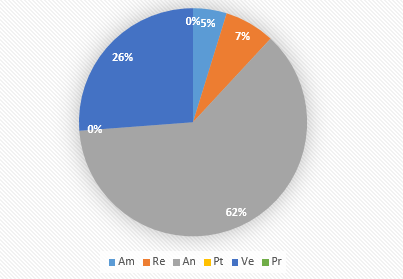
\includegraphics[scale=0.7]{PCDettaglio}
				\caption{Ore per ruolo, fase di Analisi di dettaglio.}
			\end{figure}
			%Image
			\begin{figure}[H]
				\centering
				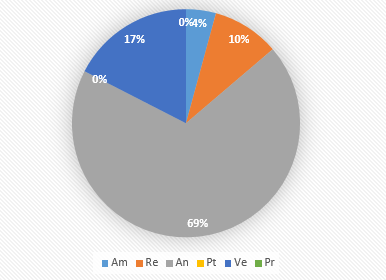
\includegraphics[scale=0.7]{PCCostiDettaglio}
				\caption{Costi per ruolo, fase di Analisi di dettaglio.}
			\end{figure}
		\section{Progettazione architetturale}
			Nelle fase di \emph{Progettazione architetturale}, le ore per ciascun ruolo sono state suddivise in questo modo:
			\begin{table}[H]
				\begin{tabularx}{\textwidth}{Y Y Y}
					\noalign{\hrule height 1.5pt}
					\rowcolor{orange!85}Ruolo & Ore & Costo \\
					\noalign{\hrule height 1.5pt}
					Responsabile & 8 & 240 \\
					Amministratore & 7 & 140 \\
					Analista & 16 & 400\\
					Progettista & 114 & 2508\\
					Verificatore & 52 & 780\\
					Programmatore & 0 & 0 \\
					\noalign{\hrule height 0.5pt}
					\textbf{Totali} & 197 & 4068 \\
					\noalign{\hrule height 1.5pt}
				\end{tabularx}
				\caption{Costo ore - fase di Progettazione architetturale. } 
				\label{TCProgettazione}
			\end{table}
			I seguenti grafici mostrano come ogni ruolo e il rispettivo costo abbiano influito sul calcolo del totale 
			costo della fase di \emph{Progettazione architetturale}.
			%Image
			\begin{figure}[H]
				\centering
				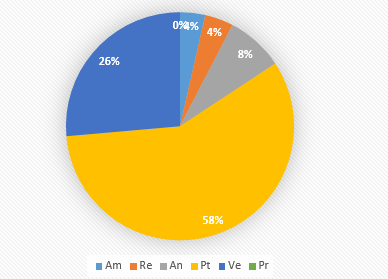
\includegraphics[scale=0.7]{PCProgettazione}
				\caption{Ore per ruolo, fase di Progettazione architetturale.}
			\end{figure}
			%Image
			\begin{figure}[H]
				\centering
				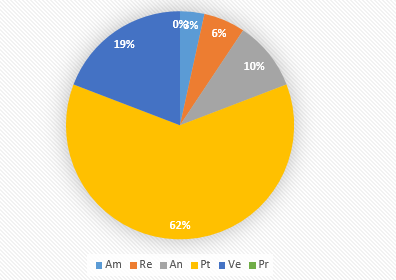
\includegraphics[scale=0.7]{PCCostiProgettazione}
				\caption{Costi per ruolo, fase di Progettazione architetturale.}
			\end{figure}
		\section{Progettazione di dettaglio e codifica}
			Nelle fase di \emph{Progettazione di dettaglio e codifica}, le ore per ciascun ruolo sono state suddivise in questo modo:
			\begin{table}[H]
				\begin{tabularx}{\textwidth}{Y Y Y}
					\noalign{\hrule height 1.5pt}
					\rowcolor{orange!85}Ruolo & Ore & Costo \\
					\noalign{\hrule height 1.5pt}
					Responsabile & 12 & 360 \\
					Amministratore & 10 & 200 \\
					Analista & 4 & 100\\
					Progettista & 101 & 2222\\
					Verificatore & 122 & 1830\\
					Programmatore & 133 & 1995 \\
					\noalign{\hrule height 0.5pt}
					\textbf{Totali} & 382 & 6707 \\
					\noalign{\hrule height 1.5pt}
				\end{tabularx}
				\caption{Costo ore - fase di Progettazione di dettaglio e codifica. }
				\label{TCCodifica}
			\end{table}
			I seguenti grafici mostrano come ogni ruolo e il rispettivo costo abbiano influito sul calcolo del totale 
			costo della fase di \emph{Progettazione di dettaglio e codifica}.
			%Image
			\begin{figure}[H]
				\centering
				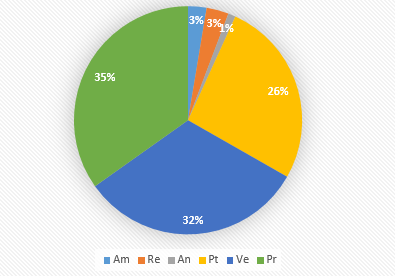
\includegraphics[scale=0.7]{PCCodifica}
				\caption{Ore per ruolo, fase di Progettazione di dettaglio e codifica.}
			\end{figure}
			%Image
			\begin{figure}[H]
				\centering
				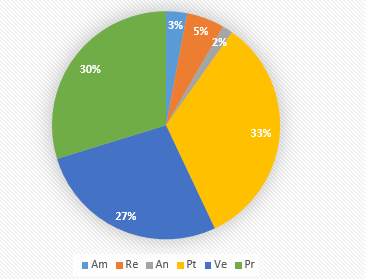
\includegraphics[scale=0.7]{PCCostiCodifica}
				\caption{Costi per ruolo, fase di Progettazione di dettaglio e codifica.}
			\end{figure}
		\section{Verifica e validazione}
			Nelle fase di \emph{Verifica e validazione}, le ore per ciascun ruolo sono state suddivise in questo modo:
			\begin{table}[H]
				\begin{tabularx}{\textwidth}{Y Y Y}
					\noalign{\hrule height 1.5pt}
					\rowcolor{orange!85}Ruolo & Ore & Costo \\
					\noalign{\hrule height 1.5pt}
					Responsabile & 5 & 150 \\
					Amministratore & 21 & 420 \\
					Analista & 0 & 0\\
					Progettista & 31 & 682\\
					Verificatore & 62 & 930\\
					Programmatore & 25 & 375 \\
					\noalign{\hrule height 0.5pt}
					\textbf{Totali} & 144 & 2557 \\
					\noalign{\hrule height 1.5pt}
				\end{tabularx}
				\caption{Costo ore - fase di Verifica e validazione. } 
				\label{TCVeV}
			\end{table}
			I seguenti grafici mostrano come ogni ruolo e il rispettivo costo abbiano influito sul calcolo del totale 
			costo della fase di \emph{Verifica e validazione}.
			%Image
			\begin{figure}[H]
				\centering
				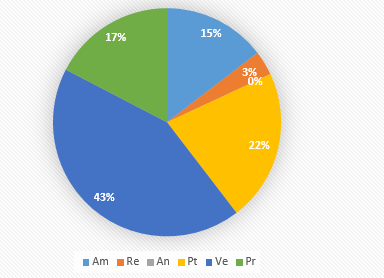
\includegraphics[scale=0.7]{PCValidazione}
				\caption{Ore per ruolo, fase di Verifica e validazione.}
			\end{figure}
			%Image
			\begin{figure}[H]
				\centering
				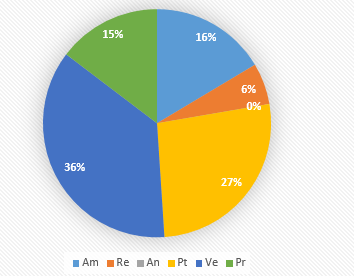
\includegraphics[scale=0.7]{PCCostiValidazione}
				\caption{Costi per ruolo, fase di Verifica e validazione.}
			\end{figure}
		\section{Totali}
			\subsection{Investimento}
				Le ore totali previste per la realizzazione del progetto sono riportate nella tabella seguente:
				\begin{table}[H]
					\begin{tabularx}{\textwidth}{Y Y Y}
						\noalign{\hrule height 1.5pt}
						\rowcolor{orange!85}Ruolo & Ore & Costo \\
						\noalign{\hrule height 1.5pt}
						Responsabile & 35 & 1050 \\
						Amministratore & 56 & 1120 \\
						Analista & 95 & 2375\\
						Progettista & 277 & 6094\\
						Verificatore & 272 & 4080\\
						Programmatore & 158 & 2370 \\
						\noalign{\hrule height 0.5pt}
						\textbf{Totali} & 893 & 17089 \\
						\noalign{\hrule height 1.5pt}
					\end{tabularx}
				\caption{Costo ore - totale con investimento. } 
				\label{TCTotaleInvestimento}
				\end{table}
				I seguenti grafici mostrano come ogni ruolo e il rispettivo costo abbiano influito sul calcolo del totale 
				costo della realizzazione del progetto.
				%Image
				\begin{figure}[H]
					\centering
					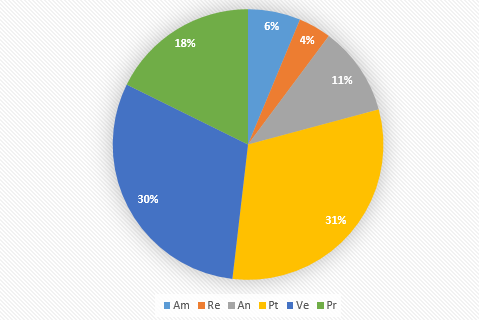
\includegraphics[scale=0.7]{PCTotali}
					\caption{Ore per ruolo, intero progetto.}
				\end{figure}
				%Image
				\begin{figure}[H]
					\centering
					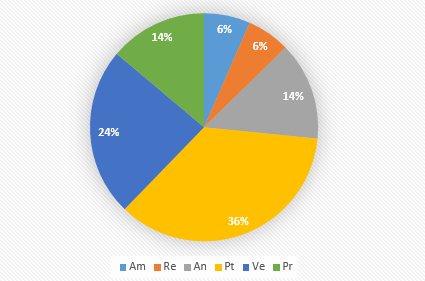
\includegraphics[scale=0.7]{PCCostiTotali}
					\caption{Costi per ruolo, intero progetto.}
				\end{figure}
			\subsection{Preventivo}
				Le ore totali previste per la realizzazione del progetto e a carico del committente sono riportate 
				nella seguente tabella:
				\begin{table}[H]
					\begin{tabularx}{\textwidth}{Y Y Y}
						\noalign{\hrule height 1.5pt}
						\rowcolor{orange!85}Ruolo & Ore & Costo \\
						\noalign{\hrule height 1.5pt}
						Responsabile & 25 & 750 \\
						Amministratore & 38 & 760 \\
						Analista & 20 & 500\\
						Progettista & 246 & 5412\\
						Verificatore & 236 & 3540\\
						Programmatore & 158 & 2370 \\
						\noalign{\hrule height 0.5pt}
						\textbf{Totali} & 723 & 13332 \\
						\noalign{\hrule height 1.5pt}
					\end{tabularx}
				\caption{Costo ore - totale rendicontate.}
				\label{TCRendicontati}
				\end{table}
				I seguenti grafici mostrano come ogni ruolo e il rispettivo costo abbiano influito sul calcolo del totale 
				costo a carico del committente
				%Image
				\begin{figure}[H]
					\centering
					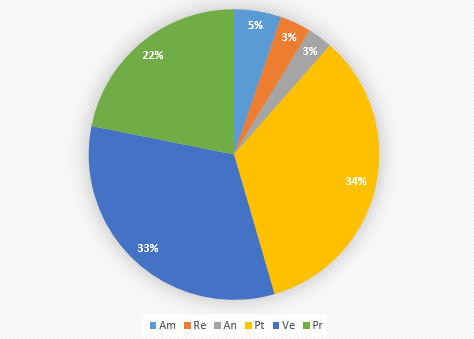
\includegraphics[scale=0.7]{PCRendicontate}
					\caption{Ore per ruolo, rendicontate.}
				\end{figure}
				%Image
				\begin{figure}[H]
					\centering
					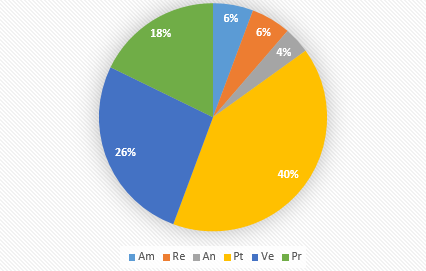
\includegraphics[scale=0.7]{PCCostiRendicontati}
					\caption{Costi per ruolo, rendicontati.}
				\end{figure}
			\subsection{Conclusione}
				Il costo totale per lo sviluppo del progetto, indicato nella \hyperref[TCRendicontati]{Tabella 4.19} viene 
				arrotondato a 13.500\euro. L'arrotondamento per eccesso è una precauzione in quanto le stime di ore di lavoro 
				necessarie per ogni task e attività potrebbero rilevarsi insufficienti. In questo modo, anche sforando di qualche 
				ora il gruppo è assicurato, e riuscirà più facilmente a rimanere all'interno dei costi preventivati.
				
				Inoltre, se uno dei rischi successivamente analizzati dovesse presentarsi, il gruppo avrà comunque a disposizione 
				un monte ore non nullo per rimediare ai danni causati dal verificarsi del rischio.
	\mychapter{5}{Analisi dei rischi}
		Al fine di migliorare l'avanzamento del progetto, è stata effettuata un'accurata analisi dei rischi suddivisa in:
		\begin{itemize}
			\item \textbf{Identificazione:} in cui si identificano i principali fattori di rischi come:
			\begin{itemize}
				\item Variabilità della disponibilità del personale;
				\item Variabilità delle tecnologie;
				\item Ritardo o mutazione di requisiti fondamentali;
				\item Specifiche in ritardo.
			\end{itemize}
			\item \textbf{Analisi:} durante la quale si individua la possibilità di occorrenza di ogni rischio, e le conseguenze a cui porterebbe.
			\item \textbf{Pianificazione:} scelta di tecniche per evitare il verificarsi dei rischi verificati, o per mitigarne gli effetti.
			\item \textbf{Controllo:} attività svolta durante tutto il ciclo di vita del progetto per prevedere il verificarsi dei rischi
			ed evitare che si verifichino.
		\end{itemize}
		Per ogni rischio individuato viene quindi stilata una lista di attributi quali: la sua probabilità di occorrenza, la gravità delle 
		conseguenze a cui porterebbe il suo verificarsi, una descrizione, le strategie da utilizzare per la sua rilevazione preventiva e le 
		contromisure da adottare (nel caso in cui il rischio si verifichi, o nel caso in cui si noti che il rischio sta per verificarsi). \\
		L'identificazione dei rischi viene gestita a livelli.
		
		\section{Livello tecnologico}
			\subsection{Tecnologie adottate}
				\subsubsection{Probabilità:}
					Bassa.
				\subsubsection{Gravità:}
					Alta.
				\subsubsection{Descrizione:}
					Nessun membro del gruppo ha una conoscenza in tutte le tecnologie utilizzate nel 
					progetto. È quindi possibile che il gruppo incontri inconvenienti nell'utilizzo 
					di determinati strumenti o tecnologie.
				\subsubsection{Contromisure:}
					L'\emph{Amministratore} è tenuto a fornire documentazione sufficiente riguardante 
					le tecnologie adottate, in tempo utile per permettere all'intero gruppo di documentarsi 
					in maniera autonoma.
			\subsection{Malfunzionamento degli strumenti utilizzati}
				\subsubsection{Probabilità:}
					Bassa.
				\subsubsection{Gravità:}
					Bassa.
				\subsubsection{Descrizione:}
					Il gruppo ha deciso di sfruttare servizi online gratuiti o software open-source per lo 
					sviluppo del progetto. È quindi da tenere in considerazione il possibile malfunzionamento 
					di host o di qualche servizio/piattaforma.
				\subsubsection{Contromisure:}
					Il gruppo si impegna ad effettuare un backup periodicamente in modo da preventivare un'eventuale 
					perdita di dati. Questo è compito del \emph{Responsabile di progetto}. La copia di backup sarà mantenuta 
					sia sul \emph{Drive} del gruppo, sia su un disco rimovibile. Tutti i membri del gruppo hanno a disposizione 
					un computer di supporto per poter rimanere operativi anche in caso di guasti hardware alle proprie macchine.
		\section{Livello del personale}
			\subsection{Inesperienza del gruppo}
				\subsubsection{Probabilità:} 
					Media.
				\subsubsection{Gravità:} 
					Media.
				\subsubsection{Descrizione:} 
					Il gruppo per lo sviluppo del progetto didattico andrà ad utilizzare una tecnologia 
					con la quale nessuno ha particolare familiarità, questo può portare a ritardi 
					nella fase di sviluppo dovuti a risoluzione di problemi di primo approccio ad una 
					nuova tecnologia non conosciuta.
				\subsubsection{Contromisure:}
					Il gruppo, per prevenire il verificarsi di questo rischio, ha stabilito di leggersi
					più di un manuale riguardante \emph{Scala}, il linguaggio di programmazione richiesto
					dal capitola d'appalto. Inoltre, il gruppo si sta già formando all'utilizzo delle
					altre tecnologie previste per il corretto svolgimento di ogni fase.
			\subsection{Variazione disponibilità}
				\subsubsection{Probabilità:}
					Media.
				\subsubsection{Gravità:} 
					Medio-alta.
				\subsubsection{Descrizione:}
					Ogni membro del gruppo ha deciso di dedicare un certo monte ore allo sviluppo del 
					progetto didattico. Questo monte ore, purtroppo, potrebbe non essere mantenuto da 
					ciascuno dei membri del gruppo, in quanto possono capitare imprevisti, o sviste.
				\subsubsection{Contromisure:}
					Il \emph{Responsabile di progetto} è tenuto ad avvisare qualsiasi membro del gruppo 
					nel caso in cui, all'avvicinarsi della terminazione di un compito a lui assegnato, 
					essi mancasse ancora di molte ore, superiori al carico giornaliero previsto. 
					
					Come già specificato, ogni membro del gruppo ha preso l'impegno di dedicare tempo 
					al progetto, e nel caso in cui qualcuno non rispetterà quanto detto, si presume 
					non sia una cosa voluta o pianificata.
			\subsection{Problemi tra componenti}
				\subsubsection{Probabilità:}
					Media.
				\subsubsection{Gravità:}
					Alta.
				\subsubsection{Descrizione:}
					SWEeneyThreads è un gruppo nato per questo progetto. Nessuno dei membri al suo interno 
					ha mai lavorato con tutti gli altri a qualche altro progetto. Inoltre, nessuno dei membri 
					del gruppo ha mai lavorato in un team così numeroso ad un progetto di questo livello. 
					Questo potrebbe portare a problemi di collaborazione, ad un carico eccessivo da parte di 
					alcuni, per sistemare una carenza da parte di altri; questo porterebbe ad avere un clima 
					poco profiquo durante lo svolgimento del progetto.
				\subsubsection{Contromisure:}
					È compito del \emph{Responsabile di progetto} monitorare la nascita di problematiche tra più 
					individui. Se questo si verificasse, è sempre compito del \emph{Responsabile di progetto} 
					cercare di organizzare il lavoro cercando di diminuire il più possibile la cooperazione 
					dei suddetti individui. 
					
					La differenza di opinioni in forte contrasto tra due individui verrà esposta al resto del 
					gruppo che deciderà, per maggioranza, la strada da intraprendere.
		\section{Livello organizzativo}
			\subsubsection{Probabilità:} 
				Media.
			\subsubsection{Gravità:}
				Alta.
			\subsubsection{Descrizione:}
				Durante la pianificazione di progetto, è possibile che la stima dei tempi, e quindi il
				preventivo, risulti errata. In particolare, una sottostima dei costi di produzione può 
				portare ad un ritardo nella consegna dei materiali previsti. 
			\subsubsection{Contromisure:}
				La caratteristiche del rischio rilevato implica il dovere, da parte di ogni membro del 
				gruppo, di controllare periodicamente lo stato dei tickets, in modo da rendersi conto 
				immediatamente di eventuali ritardi nello svolgimento di \emph{Task}. Particolare attenzione
				va posta alle attività contrassegnate come critiche. 
				
				Per le attività critiche si è deciso di inserire, già durante la loro pianificazione, delle 
				ore di slack, in modo che un eventuale ritardo non influenzi la durata totale del progetto. 
				Inoltre il preventivo fornito è maggiorato (se pur non di molto)rispetto a quello calcolato, 
				il che permette di avere delle ore bonus a disposizione in caso di ritardo.
		\section{Livello dei requisiti}
			\subsubsection{Probabilità:} 
				Media.
			\subsubsection{Gravità:}
				Media.
			\subsubsection{Descrizione:}
				Durante lo studio del capitolato e la stesura dei requisiti, è possibile che essi non vengano 
				capiti totalmente dagli analisti. È anche possibile che alcuni aspetti vengano studiati in modo 
				incompleto o peggio ancora in modo errato. Questo porterebbe a differenze tra le aspettative del 
				committente e la visione del prodotto del gruppo di lavoro.
			\subsubsection{Contromisure:}
				Per evitare che questo rischio si verifichi, durante le fasi di analisi si terranno più incontri 
				con il committente, in modo da chiarire incertezze su requisiti, o correggere errate interpretazioni 
				dei requisiti espressi. Inoltre, ogni documento verrà consegnato e valutato dal committente, ad ogni 
				revisione.
				
				Se si verificassero incongruenze tra le due visioni sul proddo, è importante che esse vengano comunicate 
				al gruppo dal committente al termine di ogni revisione, in modo che le analisi subiscano un miglioramento 
				incrementale permettendo di ottenerne di affidabili.
		\section{Livello di valutazione dei costi}
			\subsubsection{Probabilità:}
				Bassa.
			\subsubsection{Gravità:}
				Alta.
			\subsubsection{Descrizione:}
				Il costo per ora di ogni ruolo è stato definito a priori, non era compito del gruppo. Spetta invece al 
				gruppo la stima delle ore di lavoro necessarie per svolgere il progetto.
			\subsubsection{Contromisure:}
				Il preventivo è maggiorato, e anche le ore. I prezzi orari per ogni ruolo non è di pertinenza dei membri 
				del gruppo.

	\mychapter{6}{Meccanismi di controllo e rendicontazione}
		\section{Controllo}
			\subsection{Meccanismi di controllo}
				All'interno dell'ambiente di lavoro sono stati predisposti meccanismi per:
				\begin{itemize}
					\item Controllare l'andamento delle attività ed eventuali ritardi;
					\item Permettere un aggiornamento facilitato della pianificazione;
					\item Rendicontare le ore di lavoro spese nelle varie attività.
				\end{itemize}
			\subsection{Andamento delle attività}
				Per monitorare i ritardi sulle attività e acquisire maggiore esperienza per stime future si adotta la 
				funzione timer di Teamwork. Ogni componente del gruppo è invitato a tenere attivo il timer durante 
				tutto lo svolgimento delle attività a lui assegnate. In questo modo si può avere una misurazione del 
				tempo effettivo impiegato da ogni membro per svolgere le attività, che può poi essere confrontata con 
				la stima fatta a priori.
				%image
				\begin{figure}[H]
					\centering
					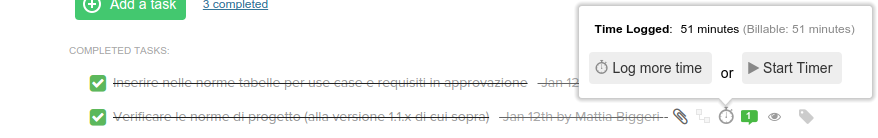
\includegraphics[scale=0.4]{teamworkTimer}
					\caption{Timer da attivare durante il lavoro svolto.}
				\end{figure}
				Inoltre per ogni attività è predisposta anche una \emph{due to date}, ovvero la data entro la quale la task deve 
				essere soddisfatta. Teamwork segnala ogni attività nel riepilogo non completata entro la data di fine con 
				una scritta rossa che riporta il ritardo. È facile per il responsabile individuare a colpo d'occhio le 
				task in ritardo e provvedere a comunicare con il/i compenti del gruppo a cui essa è assegnata per capire 
				le motivazioni del ritardo ed eventualmente rivedere le stime future.
				%image
				\begin{figure}[H]
					\centering
					
\includegraphics[scale=0.4]{teamworkTaskinRitardo}
					\caption{Visualizzazione data di scadenza di un task.}
				\end{figure}
				Se necessario è possibile impostare notifiche automatiche in prossimità o al superare di una scadenza.
				Il sistema di ticketing adottato fornisce un calendario in cui vengono indicate le date stimate di inizio e fine
				di ogni attività.\\
				Ogni membro del gruppo può consultarlo liberamente per pianificare il proprio lavoro in base agli altri
				impegni privati.
				
			\subsection{Controllo metriche di progetto}
				L'introduzione delle metriche nel progetto fornisce una maniera il più possibile oggettiva e sistematica per
				misurare le performance del gruppo. Dal punto di vista del controllo del progetto le metriche impiegate sono:
				\begin{itemize}
					\item Budget Variance
					\item Schedule Variance
				\end{itemize}
				Questi indicatori permetto al team di:
				\begin{itemize}
					\item Identificare i problemi di costo/schedulazione prima che diventino criticità;
					\item Aiutare il team a focalizzarsi sul completamento delle proprie attività.
				\end{itemize}


	\mychapter{7}{Consuntivo a finire}
		Questa sezione, lasciata per ultima perchè incrementale, riporta il prospetto economico con i 
		costi effettivamente sostenuti. Per ogni fase verrà calcolato un conguaglio, ovvero la differenza
		tra ore preventivate e spese, esso portà essere:
		\begin{itemize}
			\item \textbf{Positivo:} se il preventivo ha superato il consuntivo;
			\item \textbf{In pari:} se il preventivo e il consuntivo coincidono;
			\item \textbf{Negativo:} se il consuntivo ha superato il preventivo.
		\end{itemize}
		\section{Analisi}
			Si riporta di seguito il consuntivo della fase di \emph{Analisi}. \\
			La tabella sottostante riporta le differenze delle ore tra preventivo e consuntivo, divise per ruolo. 
			Un segno positivo indica che sono state necessarie più ore del previsto, un segno negativo indica che sono 
			state impiegate meno ore di quelle presenti nel preventivo.
						
			\begin{table}[H]
				\begin{tabularx}{\textwidth}{Y Y Y}
					\noalign{\hrule height 1.5pt}
					\rowcolor{orange!85}Ruolo & Ore & Costo \\
					\noalign{\hrule height 1.5pt}
					Responsabile & -\space 1 & -\space 30 \\
					Amministratore & 0 & 0 \\
					Analista & -\space 2 & -\space 50\\
					Progettista & +\space 1 & +\space 22\\
					Verificatore & +\space 2 & +\space 20\\
					Programmatore & 0 & 0 \\
					\noalign{\hrule height 0.5pt}
					\textbf{Totali} & 0 & -\space 38 \\
					\noalign{\hrule height 1.5pt}
				\end{tabularx}
				\caption{Differenza consuntivo/preventivo - fase di Analisi. } 
				\label{DCPAnalisi}
			\end{table}
			\subsection{Conclusioni}
				Lo svolgimento della fase di \emph{Analisi} discosta leggermente da quello programmato e 
				visualizzabile nel \emph{Gantt}. Il gruppo ha impiegato lo stesso monte ore previste, ma 
				ricoprendo ruoli diversi da quelli previsti, portando ad un conguaglio positivo.
				
				Tale differenza non influenzerà in alcun modo il costo totale del progetto in quanto le ore 
				di lavoro in questa fase non sono a carico del committente e vengono quindi emesse dal preventivo.
		%Da aggiungere man-mano
		%\section{Analisi di dettaglio}
		%\section{Progettazione architetturale}
		%\section{Progettazione di dettaglio e codifica}
		%\section{Verifica e validazione}

	\cleardoublepage
	\addcontentsline{toc}{chapter}{\listfigurename}
	\listoffigures
	
	\cleardoublepage
	\addcontentsline{toc}{chapter}{\listtablename}
	\listoftables
\end{document}
